% 第四章 Hopfion 动力学调控
\chapter{Hopfion 动力学调控}

本章围绕 Hopfion 的自旋波驱动与调控展开研究，并顺带梳理自旋转移力矩（STT）驱动的理论脉络。二维体系中，Skyrmion 在自旋波作用下的运动学已获得较充分的刻画\cite{ding2015motion,huang2023transient}，零回旋矢量的 Skyrmionium 同样能被自旋波显著驱动\cite{shen2018skyrmionium}。然而三维 Hopfion 在同类激励下的行为目前缺乏系统考察。从理论层面，Saji 等人预测了 Hopfion 所支撑的磁振子霍尔效应\cite{saji2023magnonic}；反铁磁体中，Zhang 等人则报道了 Hopfion 运动对自旋波散射的调制\cite{zhang2023magnon}。但就铁磁体系而言，自旋波直接驱动 Hopfion 的微磁学结果尚属空白。


\section{自旋转移力矩驱动的理论背景}

针对 STT 驱动下 Hopfion 的动力学，Wang 等人\cite{wang2019current}与 Liu 等人\cite{liu2020three}先后给出了系统分析。结论可归纳为一句话：轴对称 Hopfion 的回旋矢量 $\mathbf{G} = 0$，故电流作用下其沿流向做直线运动，并无霍尔偏转出现。这与二维 Skyrmion 所呈现的图像截然相反。Hopfion 的运动速度由 Thiele 方程\cref{eq:thiele}给出：
\begin{equation}
  v = \frac{u}{\alpha - \beta} \cdot \frac{\mathcal{D}_{xz}}{\mathcal{D}_{xx}}
  \label{eq:hopfion-stt-velocity}
\end{equation}
其中 $u$ 为与电流密度成正比的速度参数，$\alpha$ 和 $\beta$ 分别为 Gilbert 阻尼和非绝热 STT 系数，$\mathcal{D}$ 为耗散张量。

鉴于 $\mathbf{G} = 0$ 使 STT 驱动下的 Hopfion 呈现较为单一的直线运动模式，且相关理论与数值验证已相当充分\cite{wang2019current,liu2020three}，本文遂将动力学研究的重心转向新颖性更强的自旋波驱动路径。


\section{自旋波驱动}

作为非接触式的低热耗调控手段，自旋波驱动在能量效率上优于电流驱动。本节基于第三章确定的竞争交换铁磁体系，对自旋波传播方向与振荡方向的不同组合逐一考察其对 Hopfion 运动的影响。

\par\noindent\textbf{仿真模型与自旋波激发方案}\par\nobreak

仿真参数沿用第三章的竞争交换铁磁体系（\cref{tab:frustrated-params}），网格规模取 $100 \times 100 \times 100$，格点间距 $\SI{0.5}{nm}$。边界处理与第三章的周期性设置存在差异：此处改用\textbf{吸收边界}，即在六个面上各布置 5 格厚（约 $\SI{2.5}{nm}$）的高阻尼层，阻尼值设为 $\alpha = 100$，用以抑制反射并近似开放边界。体区阻尼则保持 $\alpha = 0.001$。

自旋波源取为 $\SI{0.5}{nm}$ 厚的薄片层，其上施加正弦振荡外磁场 $\mathbf{B}_{\text{ext}} = B_0 \sin(2\pi f t) \, \hat{n}$，默认参数为频率 $f = \SI{440}{GHz}$、振幅 $B_0 = \SI{1}{T}$。初始磁化构型选自第三章各向异性扫描中 $K_{u1} = \SI{10e3}{J/m^3}$ 对应的居中弛豫态。

Hopfion 在 $xy$ 平面内具有旋转对称性，本文据此选取 4 种代表性组合来考察自旋波的方向依赖性，具体见\cref{tab:sw-combos}。

\begin{table}[htbp]
  \centering
  \caption{自旋波驱动实验的4种组合}
  \label{tab:sw-combos}
  \begin{tabular}{cccl}
    \toprule
    编号 & 源位置 & 振荡方向 & 物理含义 \\
    \midrule
    1 & $x = -\SI{10}{nm}$ & $\hat{x}$ & 面内传播，面内振荡 \\
    2 & $x = -\SI{10}{nm}$ & $\hat{z}$ & 面内传播，面外振荡 \\
    3 & $z = -\SI{10}{nm}$ & $\hat{x}$ & 轴向传播，面内振荡 \\
    4 & $z = -\SI{10}{nm}$ & $\hat{z}$ & 轴向传播，轴向振荡 \\
    \bottomrule
  \end{tabular}
\end{table}

\par\noindent\textbf{方向选择性}\par\nobreak

5 组仿真的结果汇总于\cref{tab:drive-selection}和\cref{fig:direction-selectivity}。取 $\SI{0.5}{ns}$ 时刻 Hopfion 质心的净位移 $|\Delta r|$ 为度量，可将驱动组合划为两类：

\begin{enumerate}
  \item \textbf{有效驱动}（$|\Delta r| > \SI{1}{nm}$）：srcX\_vibX、srcY\_vibX 与 srcZ\_vibX 三组均引发了可观测的 Hopfion 迁移，其中位移最大的是 srcZ\_vibX（$|\Delta r| = \SI{6.71}{nm}$），srcX\_vibX（$\SI{2.36}{nm}$）与 srcY\_vibX（$\SI{2.31}{nm}$）次之；
  \item \textbf{无效驱动}（$|\Delta r| < \SI{0.01}{nm}$）：srcX\_vibZ 与 srcZ\_vibZ 两组下 Hopfion 基本静止，位移停留在噪声量级（$< \SI{0.006}{nm}$），相应的能量变化也仅 $\sim\SI{3e-21}{J}$，不足有效组合的 $1\%$。
\end{enumerate}

\begin{table}[htbp]
  \centering
  \caption{5 种自旋波组合的 Hopfion 驱动结果（$f = \SI{440}{GHz}$, $B_0 = \SI{1}{T}$, $t = \SI{0.5}{ns}$）}
  \label{tab:drive-selection}
  \begin{tabular}{ccrrrc}
    \toprule
    组合 & 振荡方向 & $\Delta z$ (nm) & $|\Delta r|$ (nm) & $\Delta E$ (J) & 判定 \\
    \midrule
    srcX\_vibX & $\hat{x}$ & $+2.355$ & $2.358$ & $4.15 \times 10^{-19}$ & 有效 \\
    srcX\_vibZ & $\hat{z}$ & $+0.005$ & $0.005$ & $3.38 \times 10^{-21}$ & 无效 \\
    srcY\_vibX & $\hat{x}$ & $+2.307$ & $2.310$ & $4.20 \times 10^{-19}$ & 有效 \\
    srcZ\_vibX & $\hat{x}$ & $-6.706$ & $6.706$ & $2.51 \times 10^{-19}$ & 有效 \\
    srcZ\_vibZ & $\hat{z}$ & $-0.001$ & $0.001$ & $3.24 \times 10^{-21}$ & 无效 \\
    \bottomrule
  \end{tabular}
\end{table}

\begin{figure}[htbp]
  \centering
  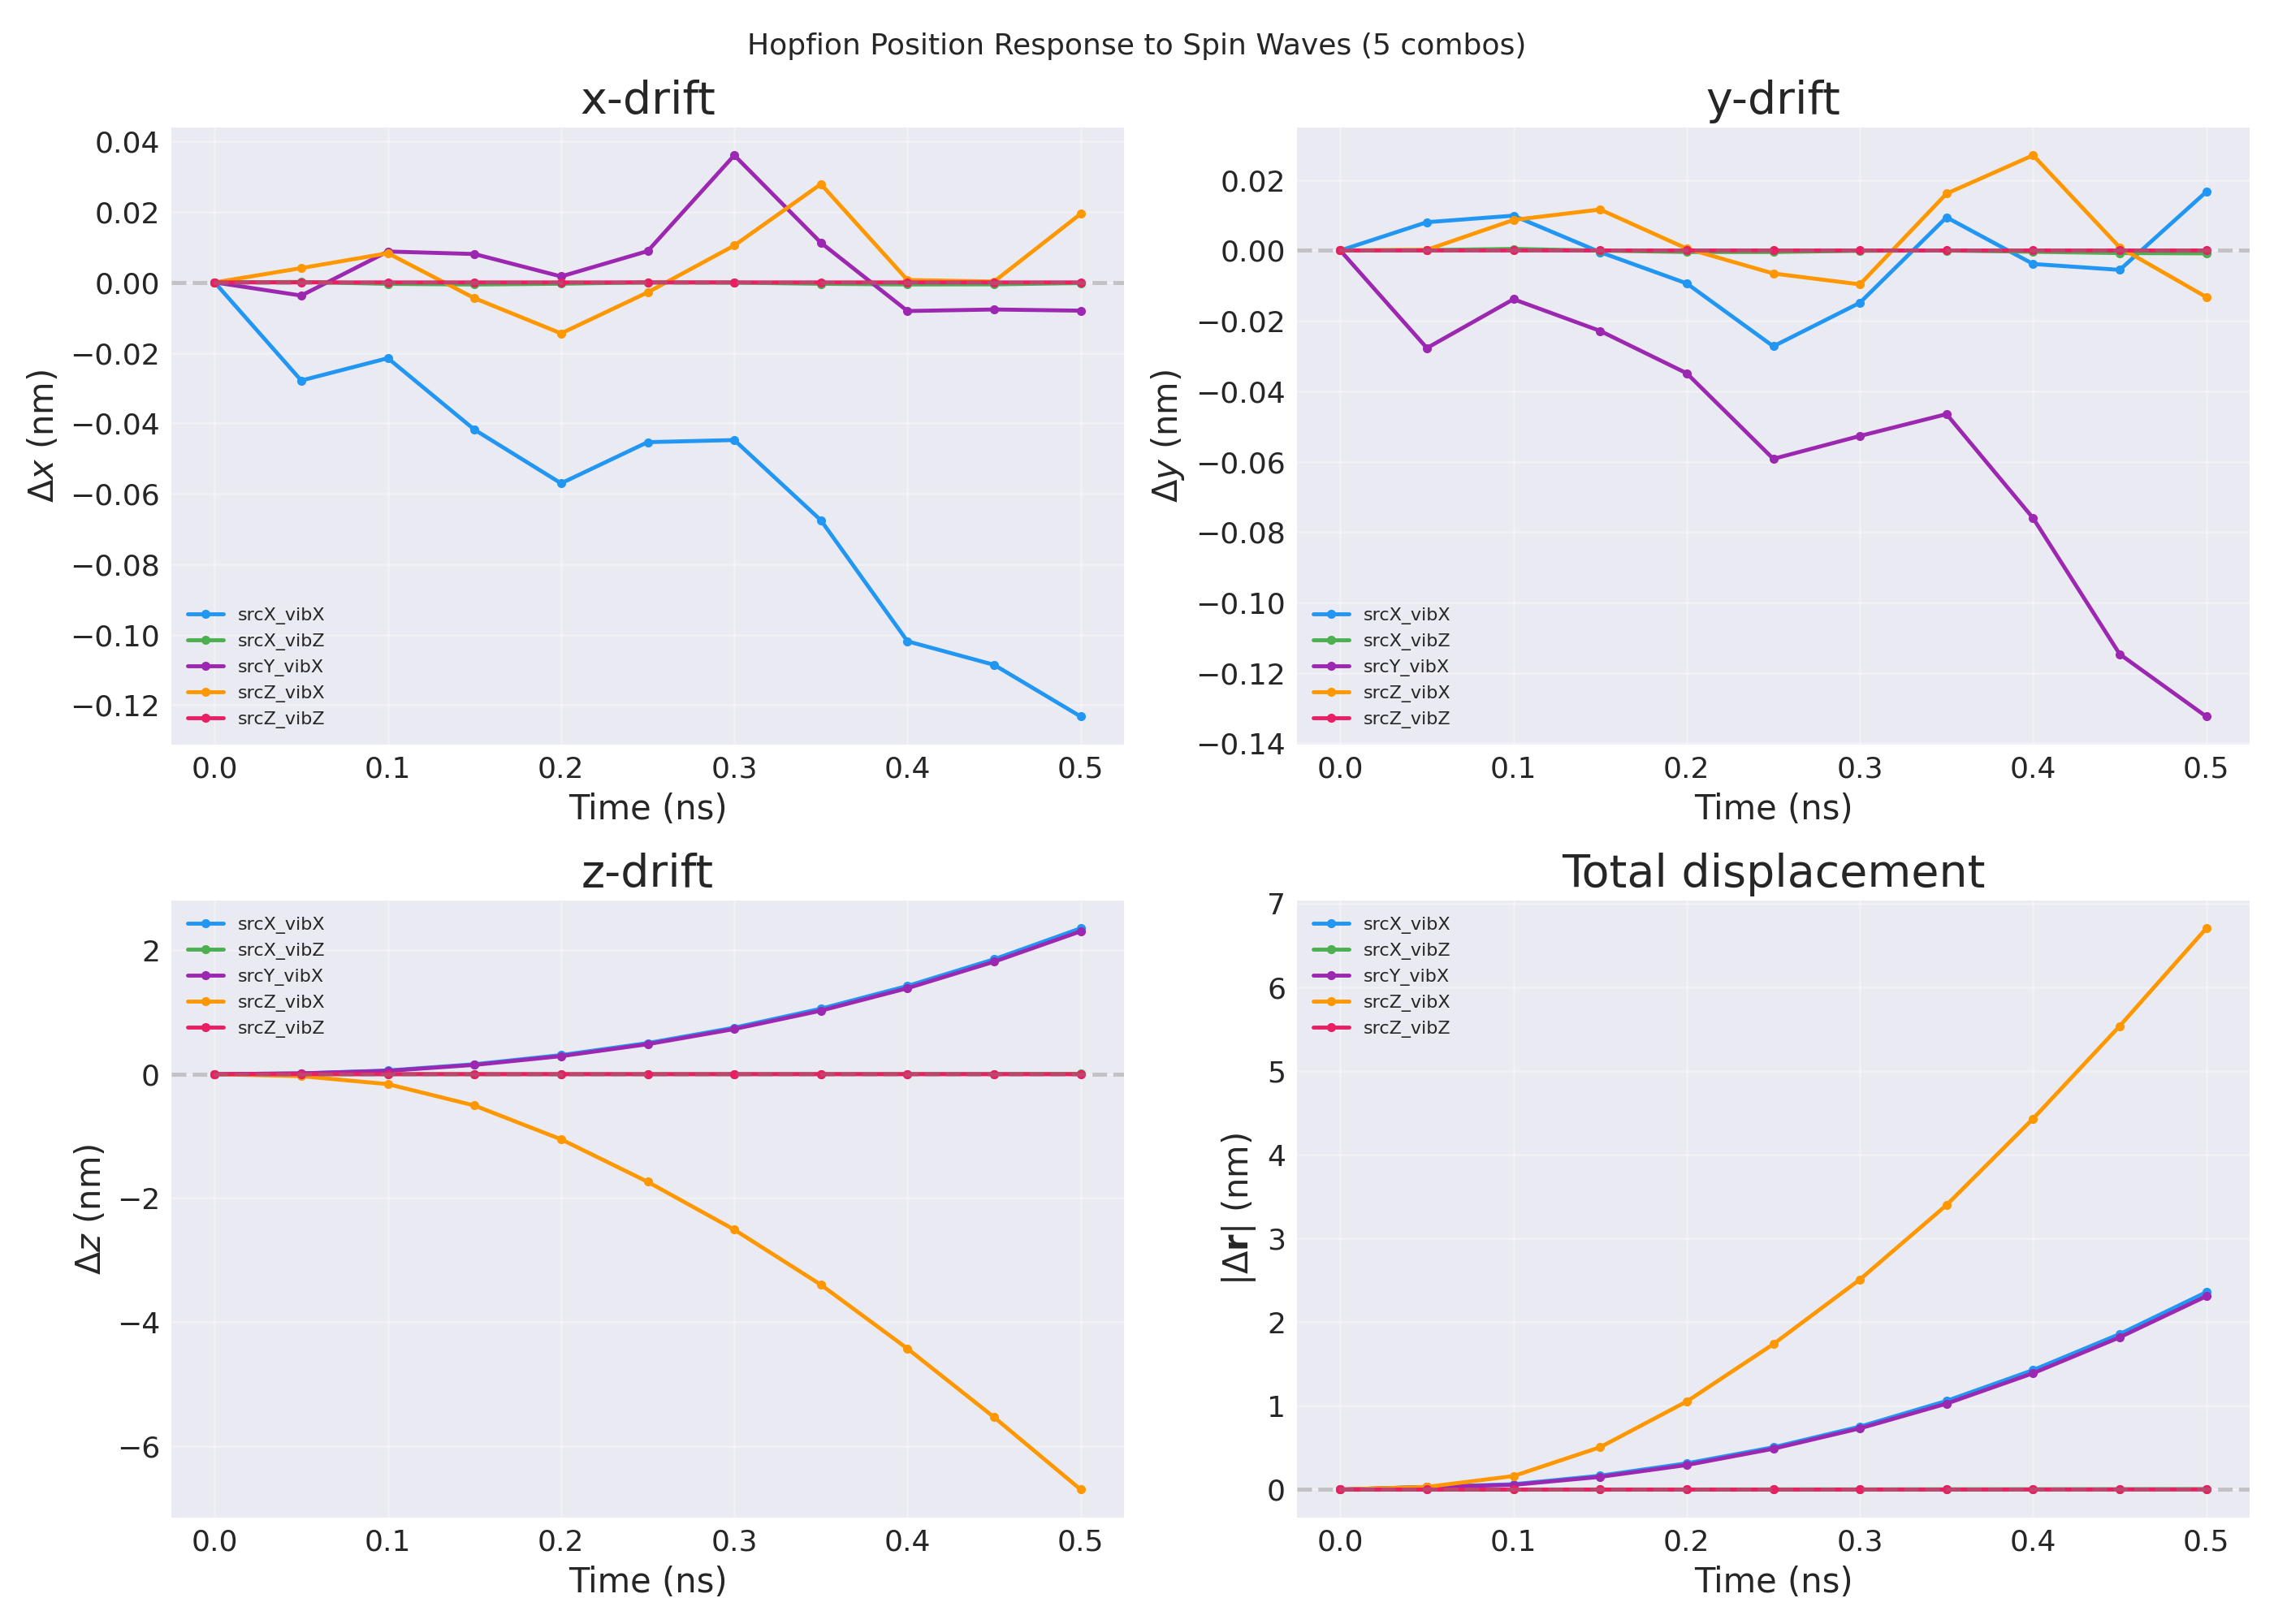
\includegraphics[width=0.95\textwidth]{figures/fig4-1_direction_selectivity.png}
  \caption{5 种驱动组合下 Hopfion 质心坐标的时间演化。面内振荡（vibX）显著推动 Hopfion 运动，面外振荡（vibZ）则未见响应}
  \label{fig:direction-selectivity}
\end{figure}

由上述结果可提炼出两点。\textbf{（1）振荡方向选择性}：真正能推动 Hopfion 的仅限于 $\hat{x}$ 方向的面内振荡，$\hat{z}$ 方向的面外振荡几乎不起作用。物理原因在于 $\hat{z}$ 振荡未破坏 Hopfion 的轴对称性，无法把能量注入到平动自由度；$\hat{x}$ 振荡则打破了面内对称，从而为平动提供线性动量。\textbf{（2）面内等价性}：srcX\_vibX 与 srcY\_vibX 的位移量级几近一致（$2.36$ 对 $\SI{2.31}{nm}$），再度印证了 Hopfion 面内传播的各向同性——这与其 $xy$ 面旋转不变性相符。

从仿真结果来看，三个有效组合在方向上也呈现系统性分化。srcX\_vibX、srcY\_vibX 推动 Hopfion 朝 $+z$ 运动，方向与传播方向垂直；srcZ\_vibX 则驱使其沿 $-z$ 运动，与传播方向共线。此类方向对比正是后续双向轴向控制方案的物理基础。

\par\noindent\textbf{频率响应谱}\par\nobreak

既已锁定面内振荡（vibX）为有效驱动形式，本文随即对面内传播（srcX）与轴向传播（srcZ）分别开展频率扫描，以刻画 Hopfion 运动的频率依赖关系。

\subsubsection{面内传播 srcX 的频率响应}

采用 srcX\_vibX 组合，幅度固定为 $B_0 = \SI{1}{T}$，在 $\SIrange{100}{1000}{GHz}$ 区间内以 $\SI{100}{GHz}$ 为步长扫描 10 个频率点。各频率对应的 Hopfion 运动模式分类结果见\cref{fig:srcX-motion-mode}。

\begin{figure}[htbp]
  \centering
  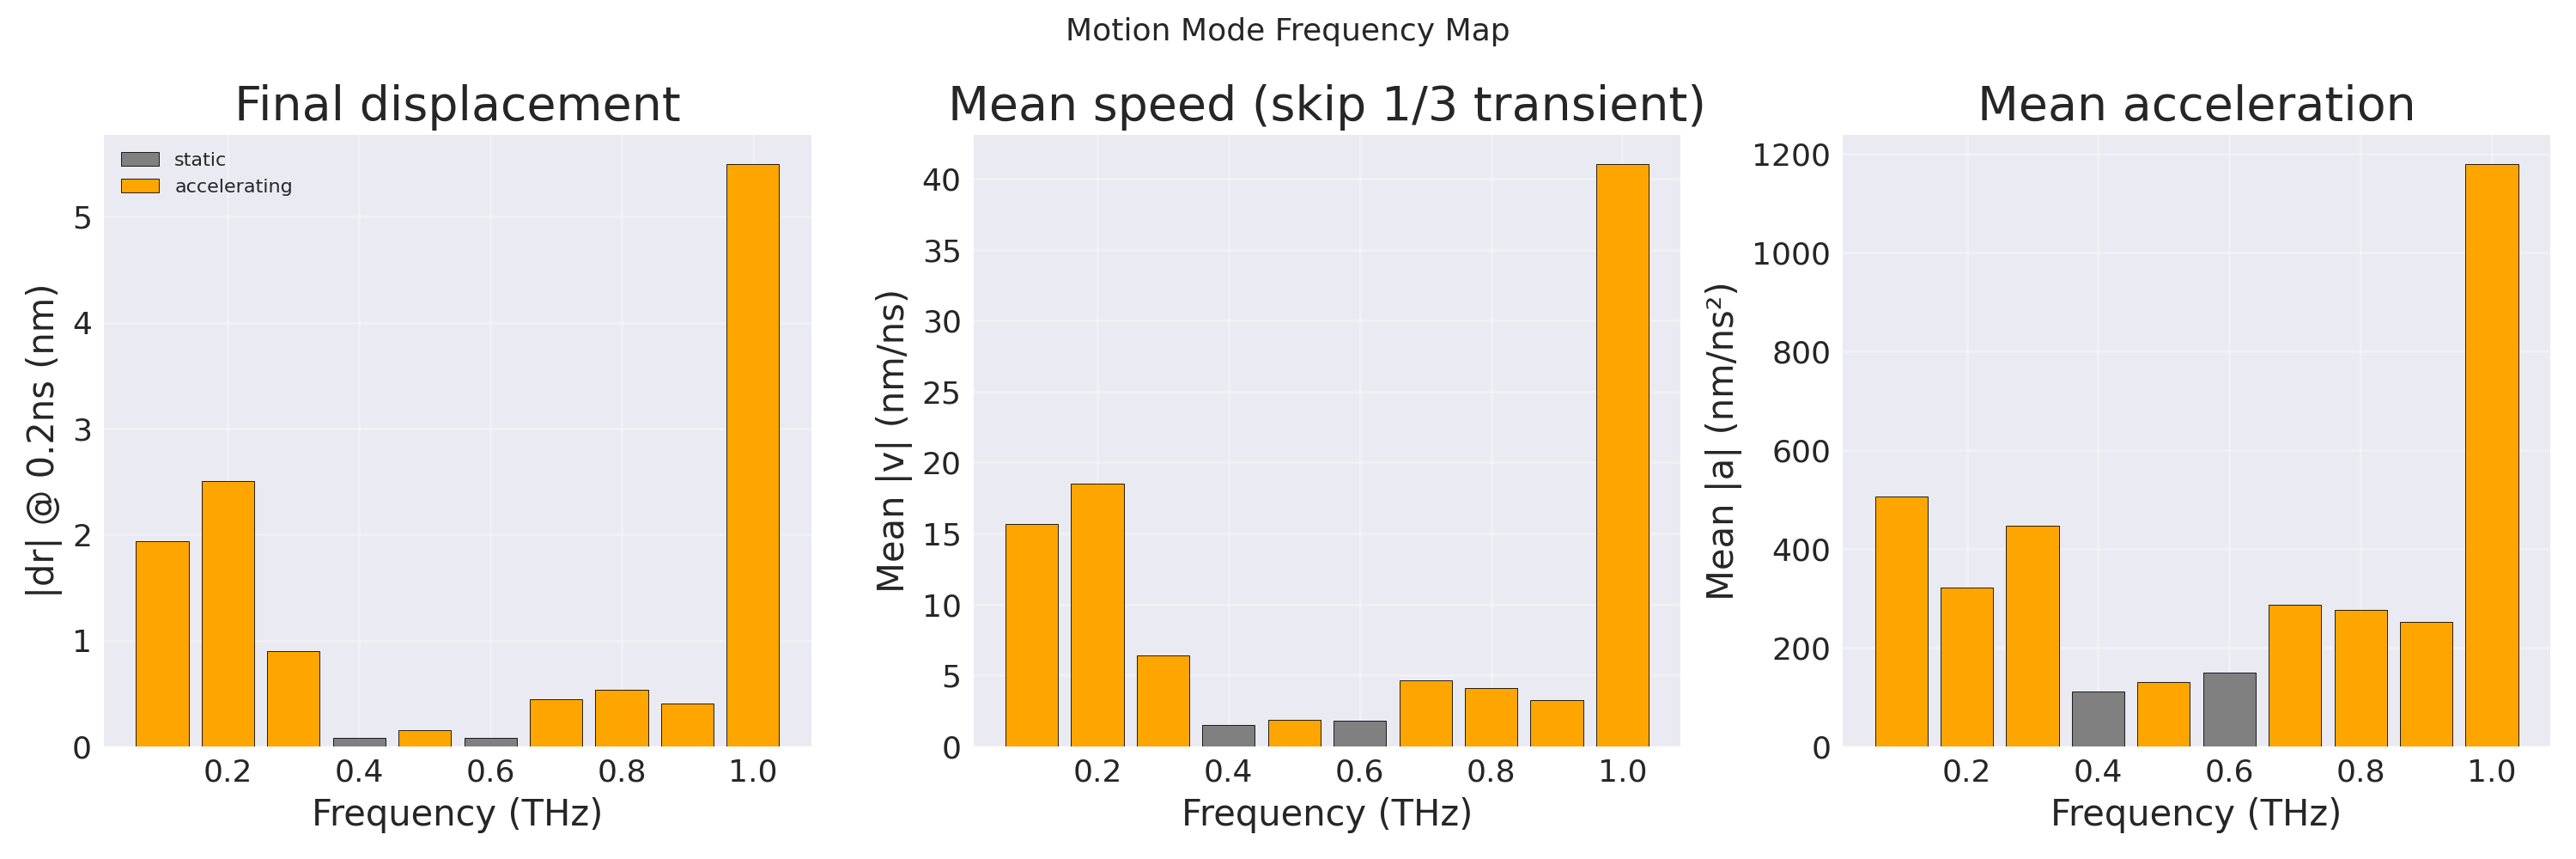
\includegraphics[width=0.95\textwidth]{figures/fig4-2_srcX_motion_mode.png}
  \caption{srcX 驱动下 10 个频率点的运动模式分类结果。蓝色实线给出 $z$ 方向位移 $\Delta z(t)$，红色虚线为相应运动模式的拟合曲线}
  \label{fig:srcX-motion-mode}
\end{figure}

\begin{figure}[htbp]
  \centering
  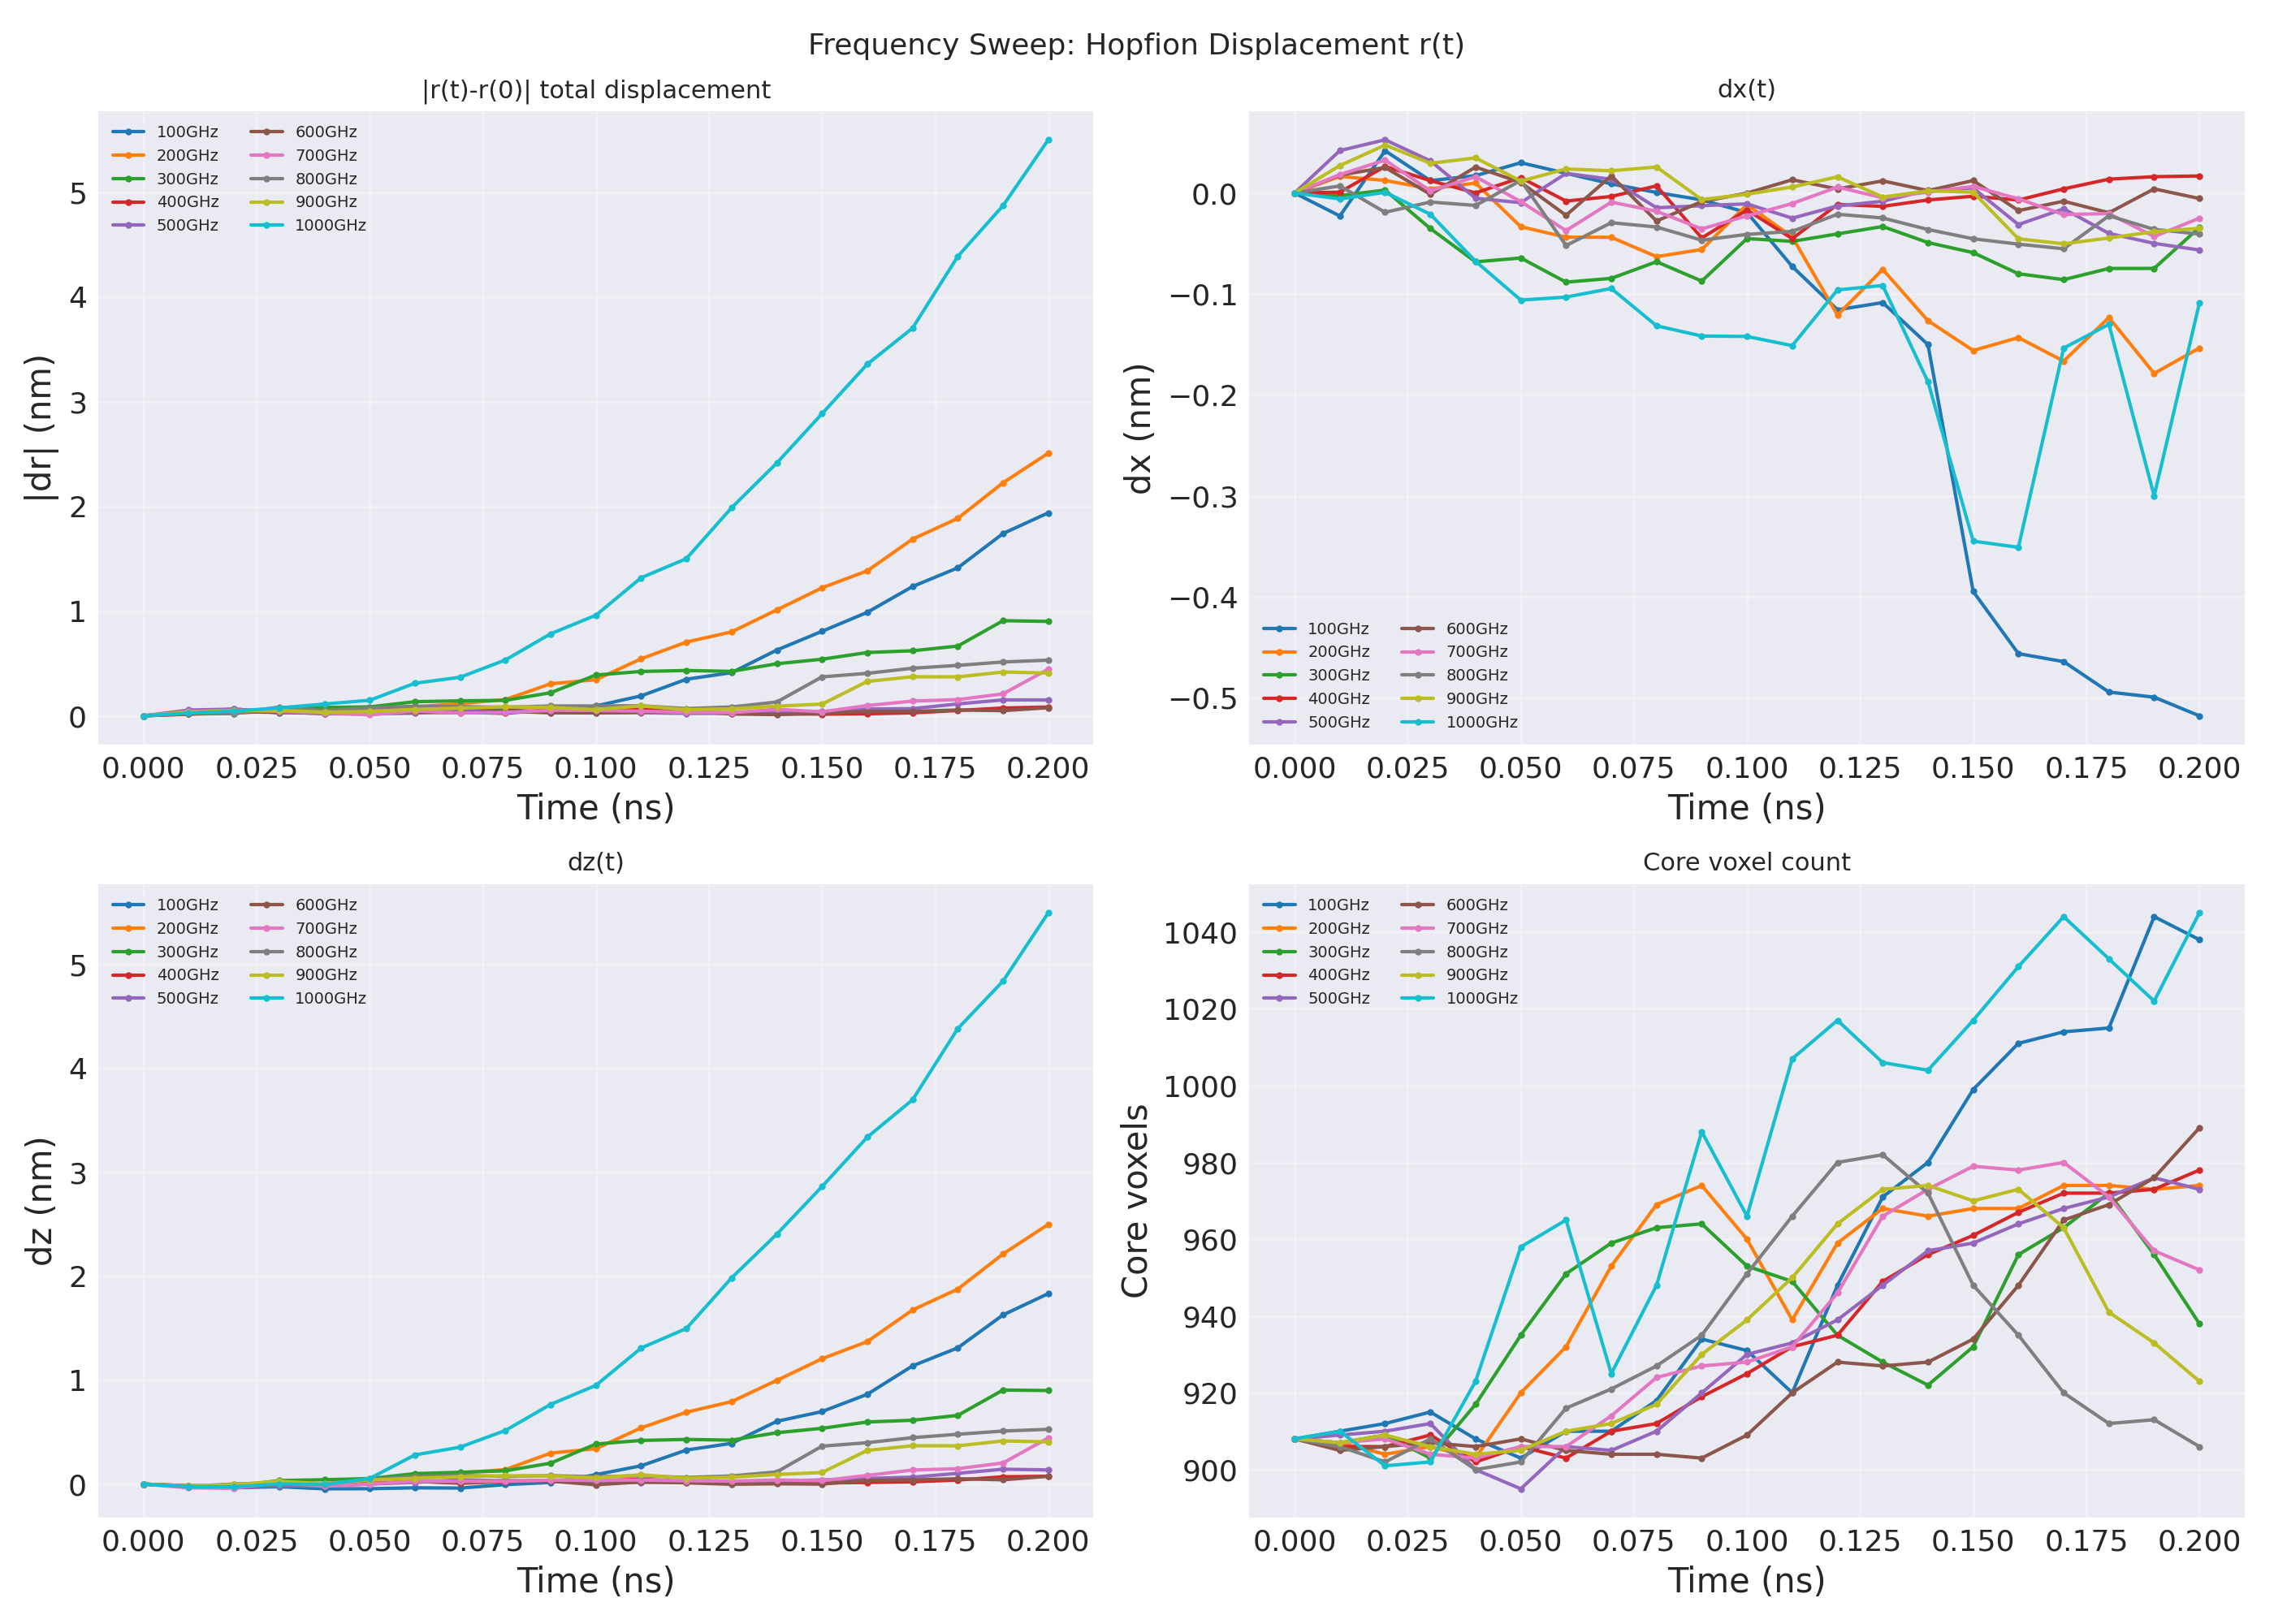
\includegraphics[width=0.95\textwidth]{figures/fig4-3_srcX_displacement.png}
  \caption{srcX 驱动下 Hopfion 位移 $|\Delta r|$ 与平均速度 $\bar{v}$ 的频率依赖关系。最强响应出现在 $\SI{1000}{GHz}$，$\SIrange{400}{600}{GHz}$ 为死区}
  \label{fig:srcX-displacement}
\end{figure}

响应呈现出显著的频率选择性。低频段 $\SIrange{100}{200}{GHz}$（$|\Delta r| = \SIrange{1.94}{2.51}{nm}$）与 $\SI{1000}{GHz}$（$|\Delta r| = \SI{5.50}{nm}$，全频段峰值）共同构成\textbf{有效驱动区}。\textbf{死区}落在 $\SIrange{400}{600}{GHz}$（$|\Delta r| < \SI{0.15}{nm}$），Hopfion 近乎静止；$\SIrange{700}{900}{GHz}$ 的中间段响应介于两者之间（$\SIrange{0.4}{0.5}{nm}$）。需要指出的是，所有频率下 Hopfion 均沿 $+z$ 方向迁移，运动方向与频率无关。

\subsubsection{轴向传播 srcZ 的频率响应}

对于 srcZ 驱动，本文将频率扫描延伸至 $\SIrange{25}{1500}{GHz}$，采取"粗扫+细化"的方式共覆盖 20 个点。相应的结果由\cref{fig:srcZ-freq-response}和\cref{fig:srcZ-direction-map}给出。

\begin{figure}[htbp]
  \centering
  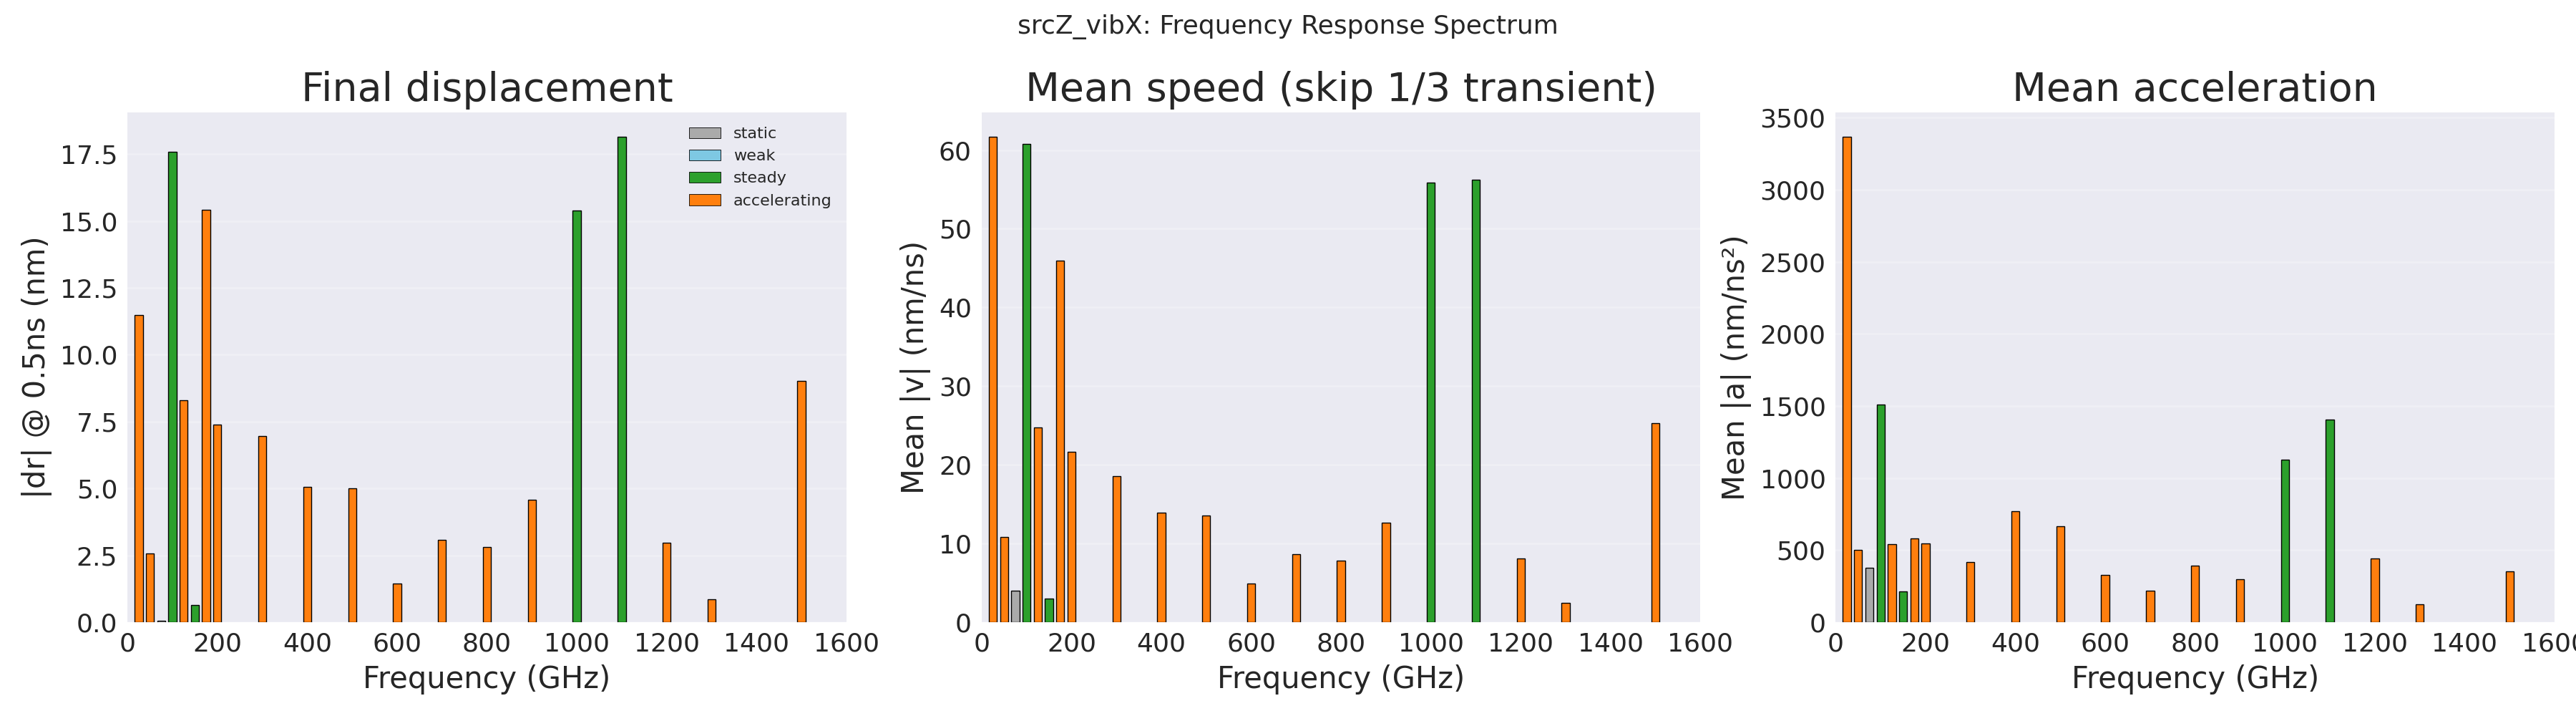
\includegraphics[width=0.95\textwidth]{figures/fig4-4_srcZ_freq_response.png}
  \caption{srcZ 驱动下 20 个频率点的 Hopfion 位移谱。全频段最强响应出现在 $\SI{1100}{GHz}$（$|\Delta r| = \SI{18.1}{nm}$），$\SI{100}{GHz}$ 则是仅有的一个 $+z$ 异常点}
  \label{fig:srcZ-freq-response}
\end{figure}

\begin{figure}[htbp]
  \centering
  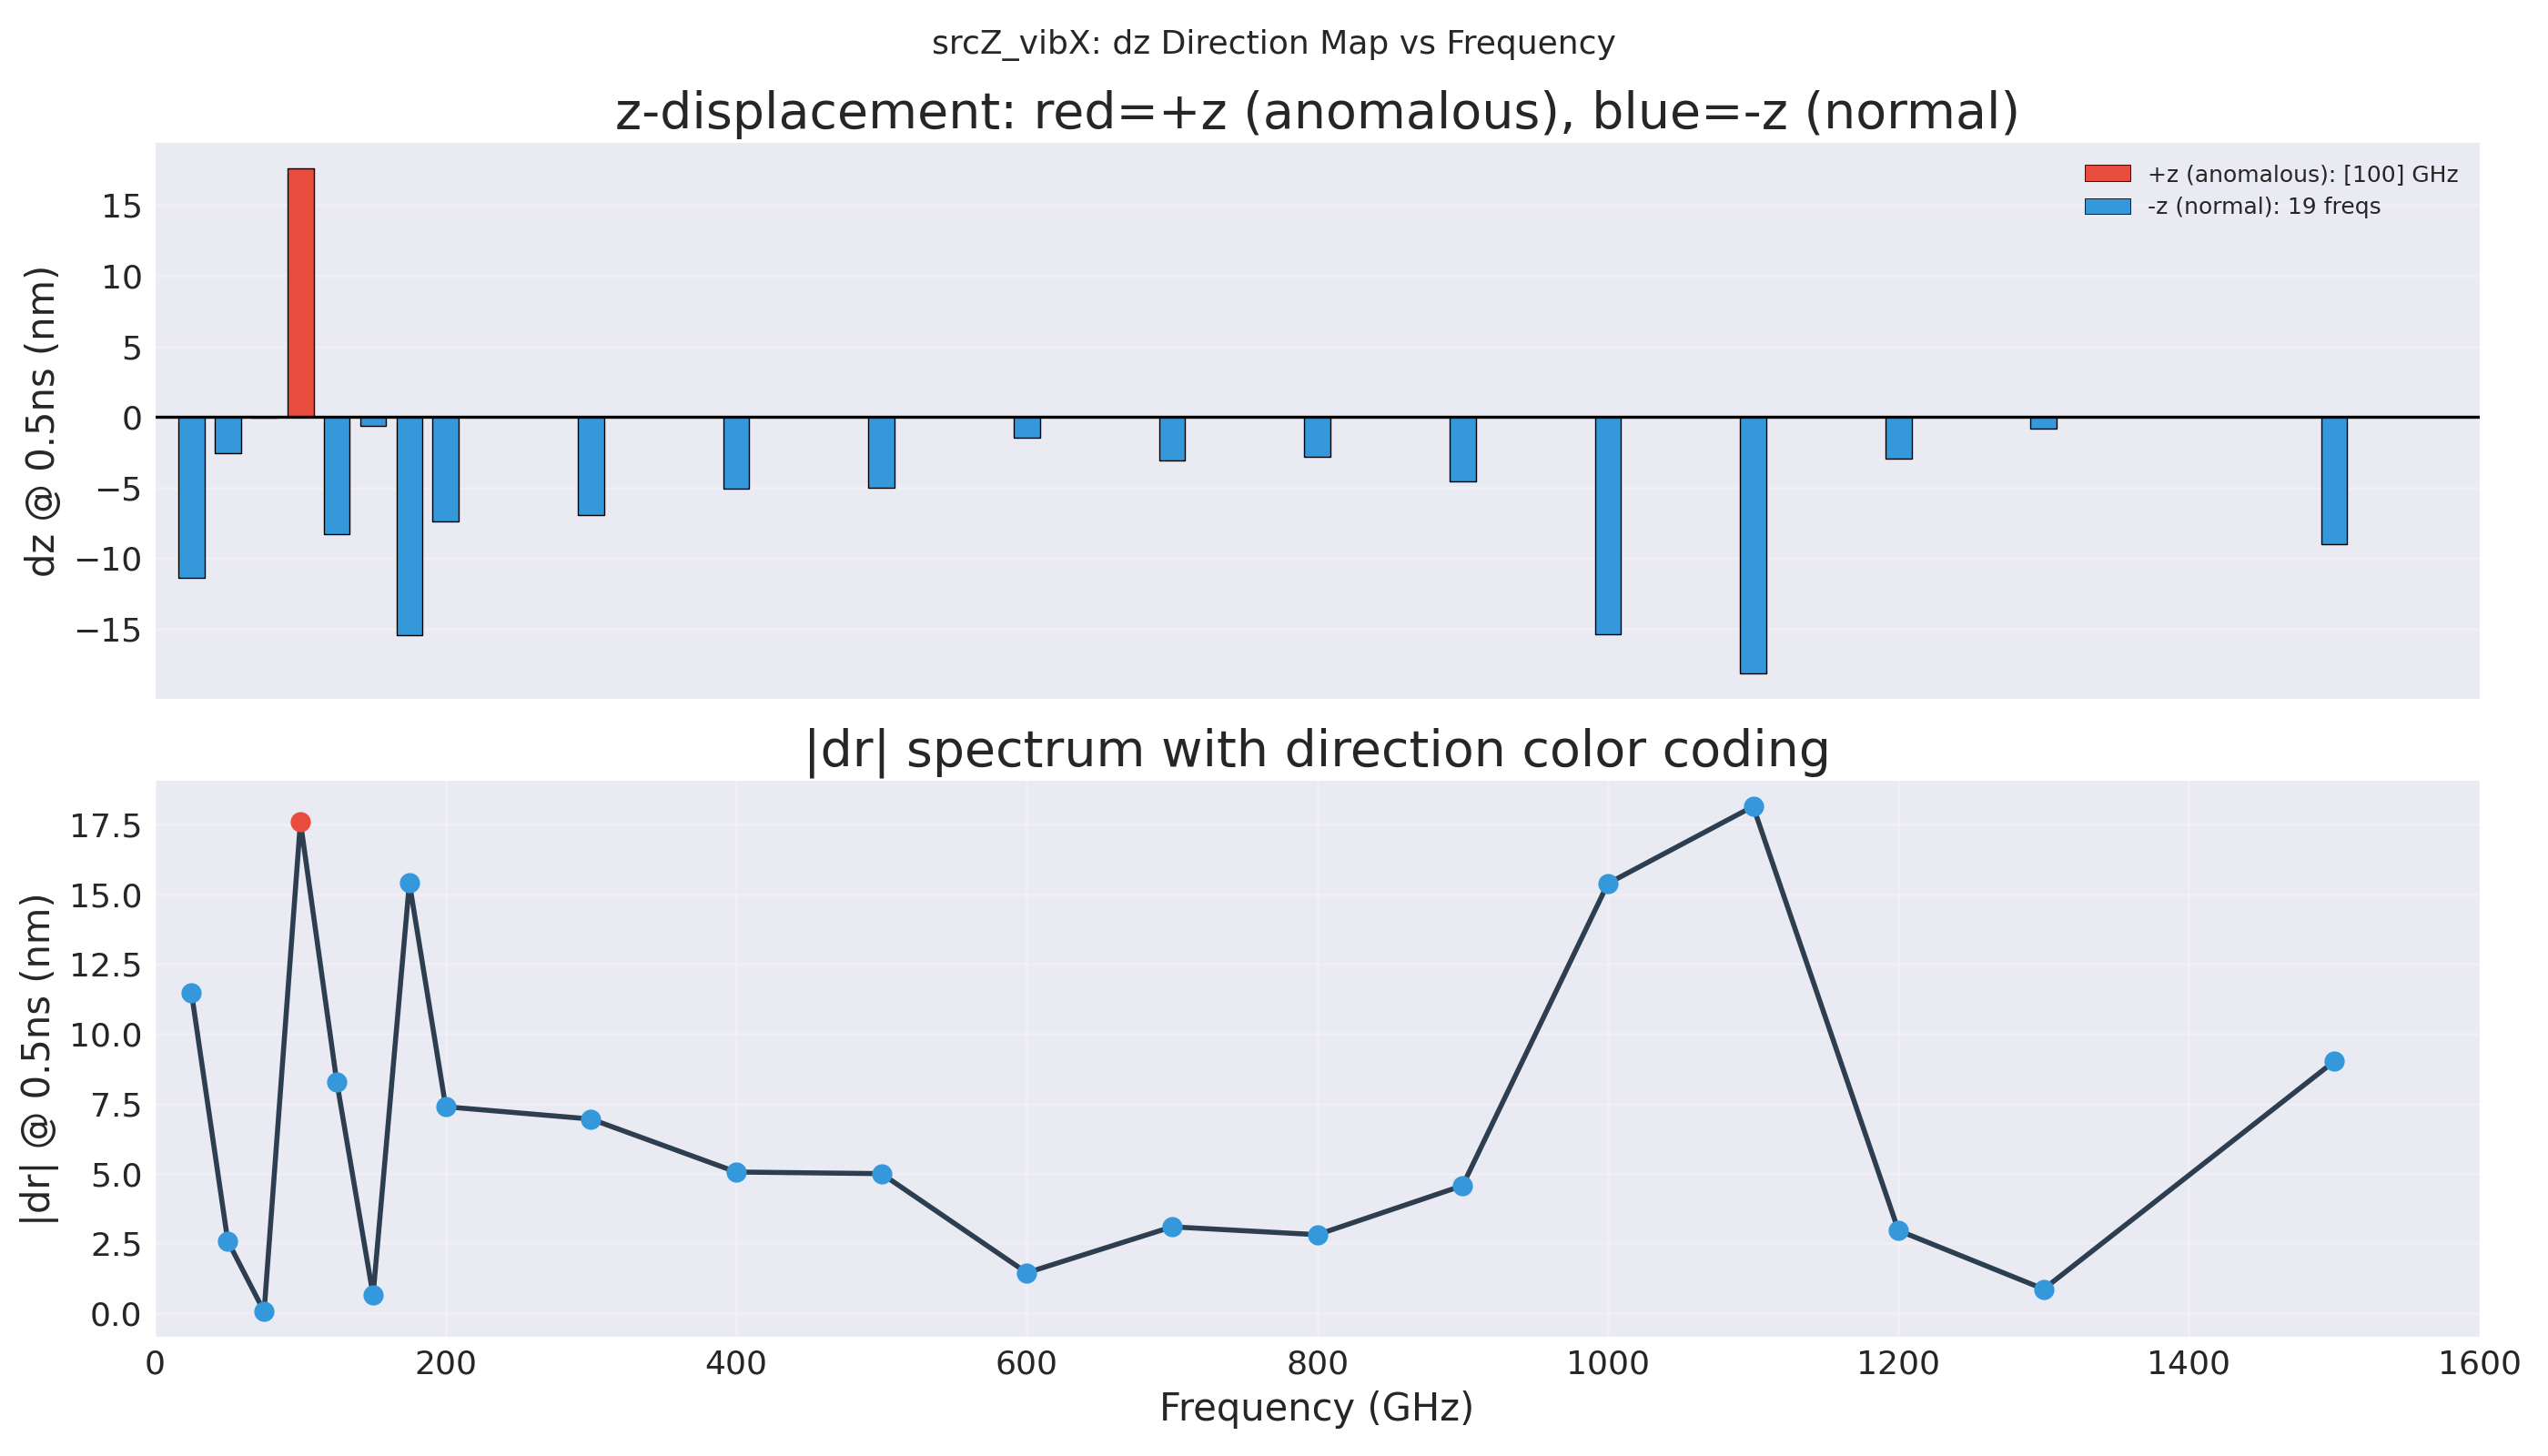
\includegraphics[width=0.95\textwidth]{figures/fig4-5_srcZ_direction_map.png}
  \caption{srcZ 驱动的方向分布图。除 $\SI{100}{GHz}$ 以外，其余各频率下 Hopfion 均沿 $-z$ 方向运动}
  \label{fig:srcZ-direction-map}
\end{figure}

srcZ 的频率响应与 srcX 形成鲜明对照，其特征可概括为三方面：（1）\textbf{方向异常}：$\SI{100}{GHz}$ 为唯一的 $+z$（朝向源）驱动频率（$\Delta z = +\SI{17.6}{nm}$），剩余 19 个频率点全部驱使 Hopfion 沿 $-z$（远离源）迁移。（2）\textbf{共振谱多峰}：全局最强共振出现在 $\SI{1100}{GHz}$（$|\Delta r| = \SI{18.1}{nm}$，$\bar{v} = \SI{56.3}{nm/ns}$），$\SI{100}{GHz}$（$\SI{17.6}{nm}$）与 $\SI{1000}{GHz}$（$\SI{15.4}{nm}$）构成次强峰；死区则分布于 $\SI{75}{GHz}$、$\SI{150}{GHz}$、$\SI{600}{GHz}$ 与 $\SI{1300}{GHz}$。（3）\textbf{运动模式}：强响应点以"steady"模式（匀速）运动为主，弱响应点则呈"accelerating"加速图像。

srcX 与 srcZ 的响应差别折射出不同传播方向与 Hopfion 内模耦合通道的差异。面内传播的自旋波主要激活面内平动模式，从而产生 $+z$ 方向的 Hall 式迁移；轴向传播则直接耦合到轴向平动通道，对应 $-z$ 方向运动，二者的共振频率分布也因此互不相同。

\par\noindent\textbf{能量吸收谱}\par\nobreak

为从定量层面评估 Hopfion 与自旋波的耦合强度，本文从仿真记录的总能量 $E_{\text{total}}(t)$ 中提取能量吸收率 $\mathrm{d}E/\mathrm{d}t$。具体做法是在 $0.3T$–$T$ 时段（绕过初始瞬态）对能量曲线做线性拟合，所得斜率即对应频率点的平均吸收率。

\begin{figure}[htbp]
  \centering
  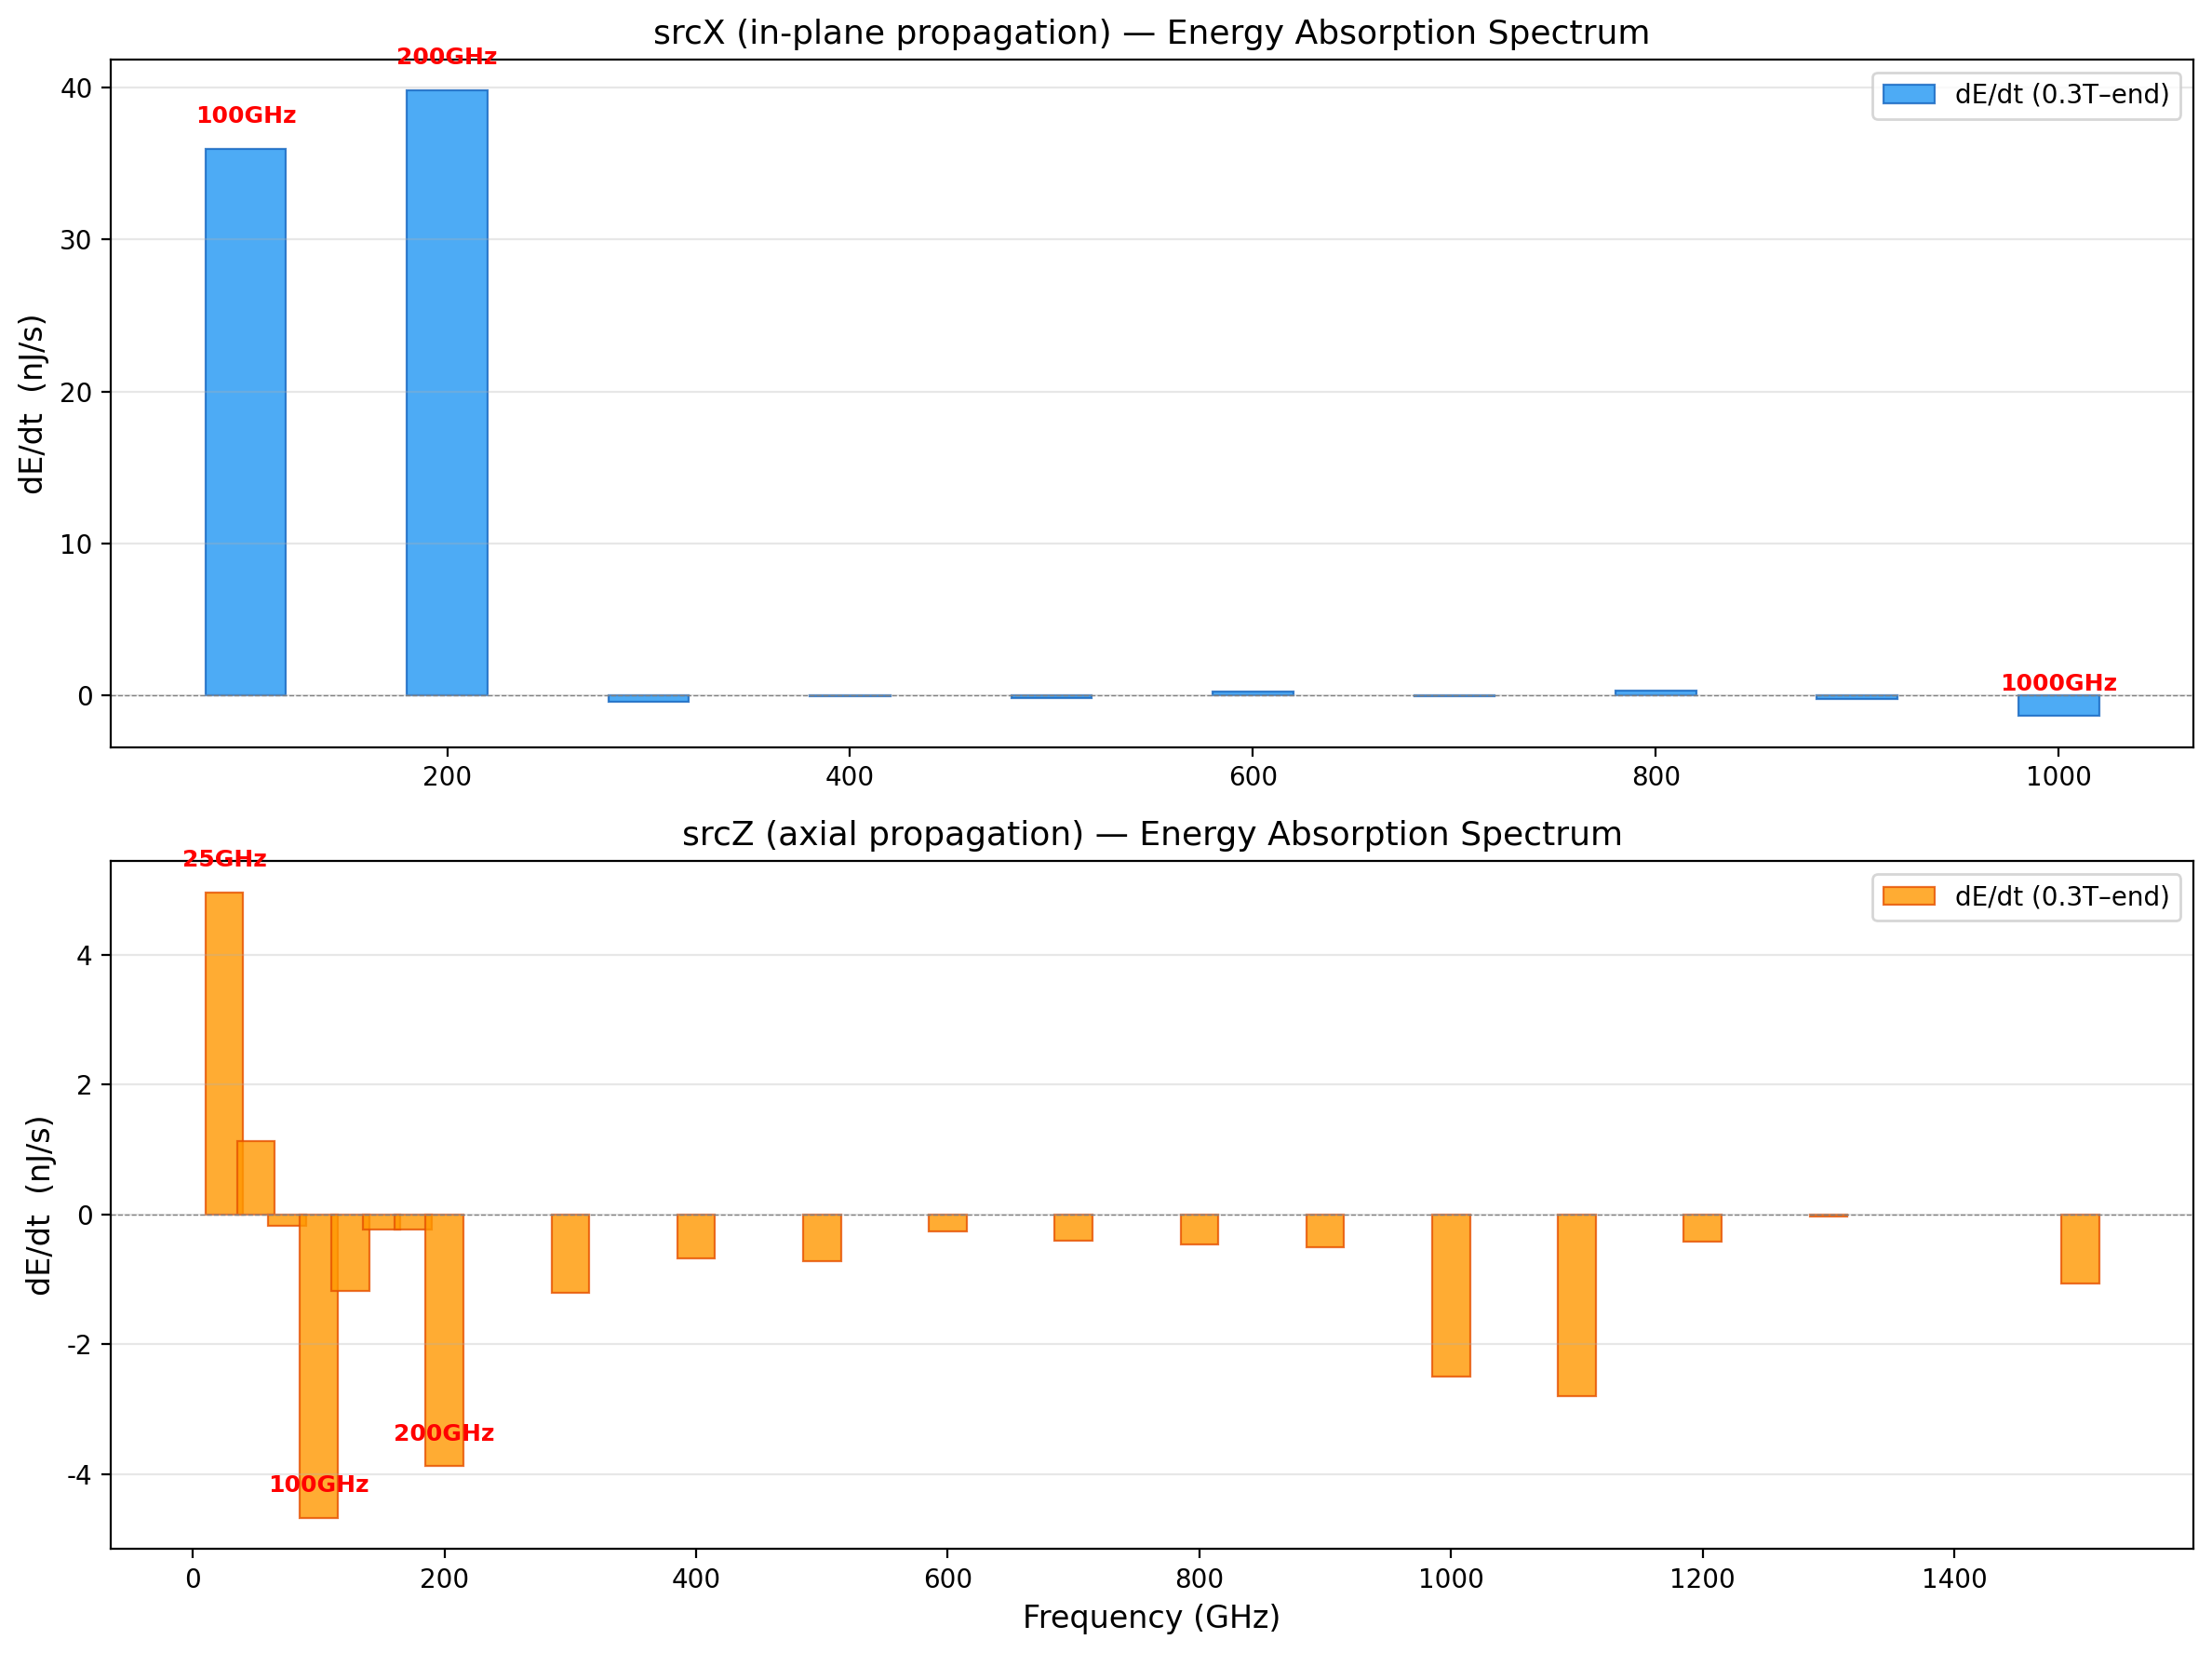
\includegraphics[width=0.95\textwidth]{figures/fig4-6_energy_absorption.png}
  \caption{能量吸收谱 $\mathrm{d}E/\mathrm{d}t$ 随频率 $f$ 的变化。上图为 srcX（面内传播），峰值位于 $\SI{200}{GHz}$；下图为 srcZ（轴向传播），最强吸收出现在 $\SI{100}{GHz}$}
  \label{fig:energy-absorption}
\end{figure}

由\cref{fig:energy-absorption}可见，srcX 的吸收谱呈现 $\SI{100}{GHz}$（$\SI{36.0}{nJ/s}$）与 $\SI{200}{GHz}$（$\SI{39.8}{nJ/s}$，$R^2 = 0.986$）的双峰结构，$\SIrange{300}{800}{GHz}$ 吸收率近乎为零（$< \SI{0.5}{nJ/s}$），与位移谱中的 $\SIrange{400}{600}{GHz}$ 死区相吻合。srcZ 的谱线则呈现非对称的多峰形态，绝对值最大者位于 $\SI{100}{GHz}$（$-\SI{4.67}{nJ/s}$，负号表示能量由系统返还给驱动场）；$\SIrange{400}{900}{GHz}$ 段维持较为稳定的吸收（$\SIrange{0.3}{0.7}{nJ/s}$）。

将吸收谱与位移谱放在一起比较，可得两点观察。其一，吸收高并不等于位移大：srcX@$\SI{200}{GHz}$ 的吸收率居首，但位移（$\SI{2.51}{nm}$）明显低于 $\SI{1000}{GHz}$ 的 $\SI{5.50}{nm}$，这表明 $\SI{1000}{GHz}$ 模式的能量-动能转换效率更高。其二，srcZ@$\SI{100}{GHz}$ 出现负吸收率，与该频率下 $+z$ 的异常运动方向相关，暗示此模式涉及的耦合机制或不同于其余频率。

\par\noindent\textbf{幅度标度律}\par\nobreak

本文将组合固定为 srcX\_vibX、频率锁定为 $f = \SI{440}{GHz}$，在 $B_0 = \SIrange{0.05}{2.0}{T}$ 内选取 6 个幅度点开展扫描，以量化 Hopfion 运动速度对驱动幅度的依赖。

\begin{figure}[htbp]
  \centering
  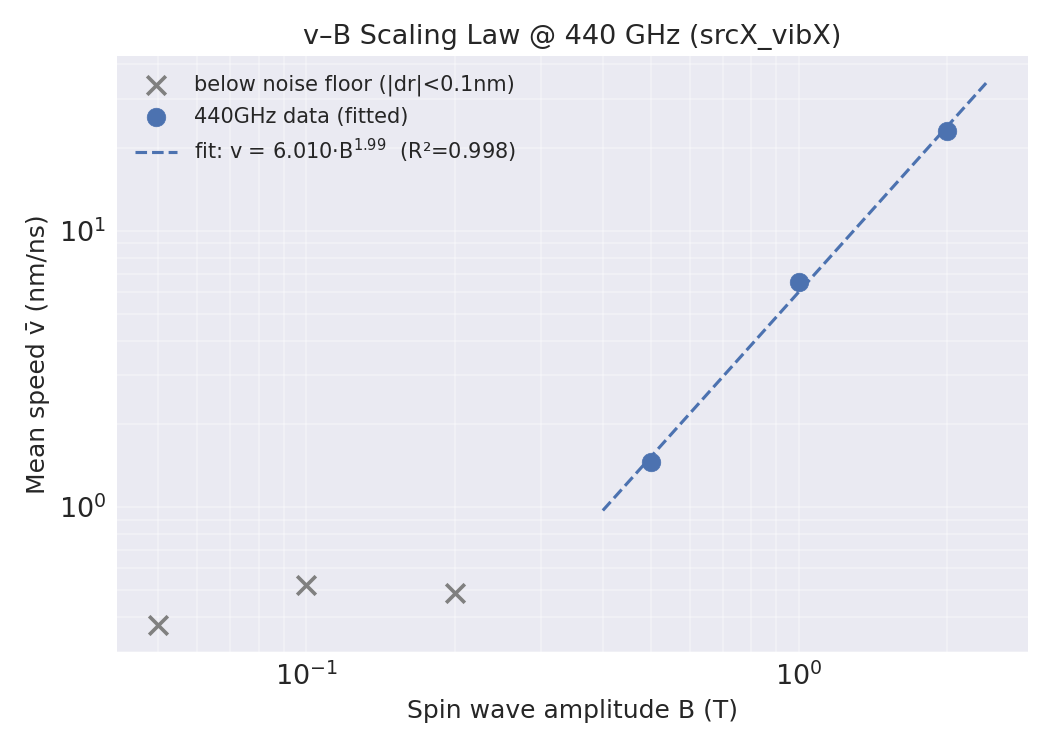
\includegraphics[width=0.95\textwidth]{figures/fig4-7_amplitude_scaling.png}
  \caption{log-log 坐标下 Hopfion 平均速度 $\bar{v}$ 对自旋波幅度 $B_0$ 的依赖关系。$B_0 \geq \SI{0.5}{T}$ 的数据段拟合给出 $\bar{v} \propto B_0^{1.99}$，$R^2 = 0.998$}
  \label{fig:amplitude-scaling}
\end{figure}

\begin{figure}[htbp]
  \centering
  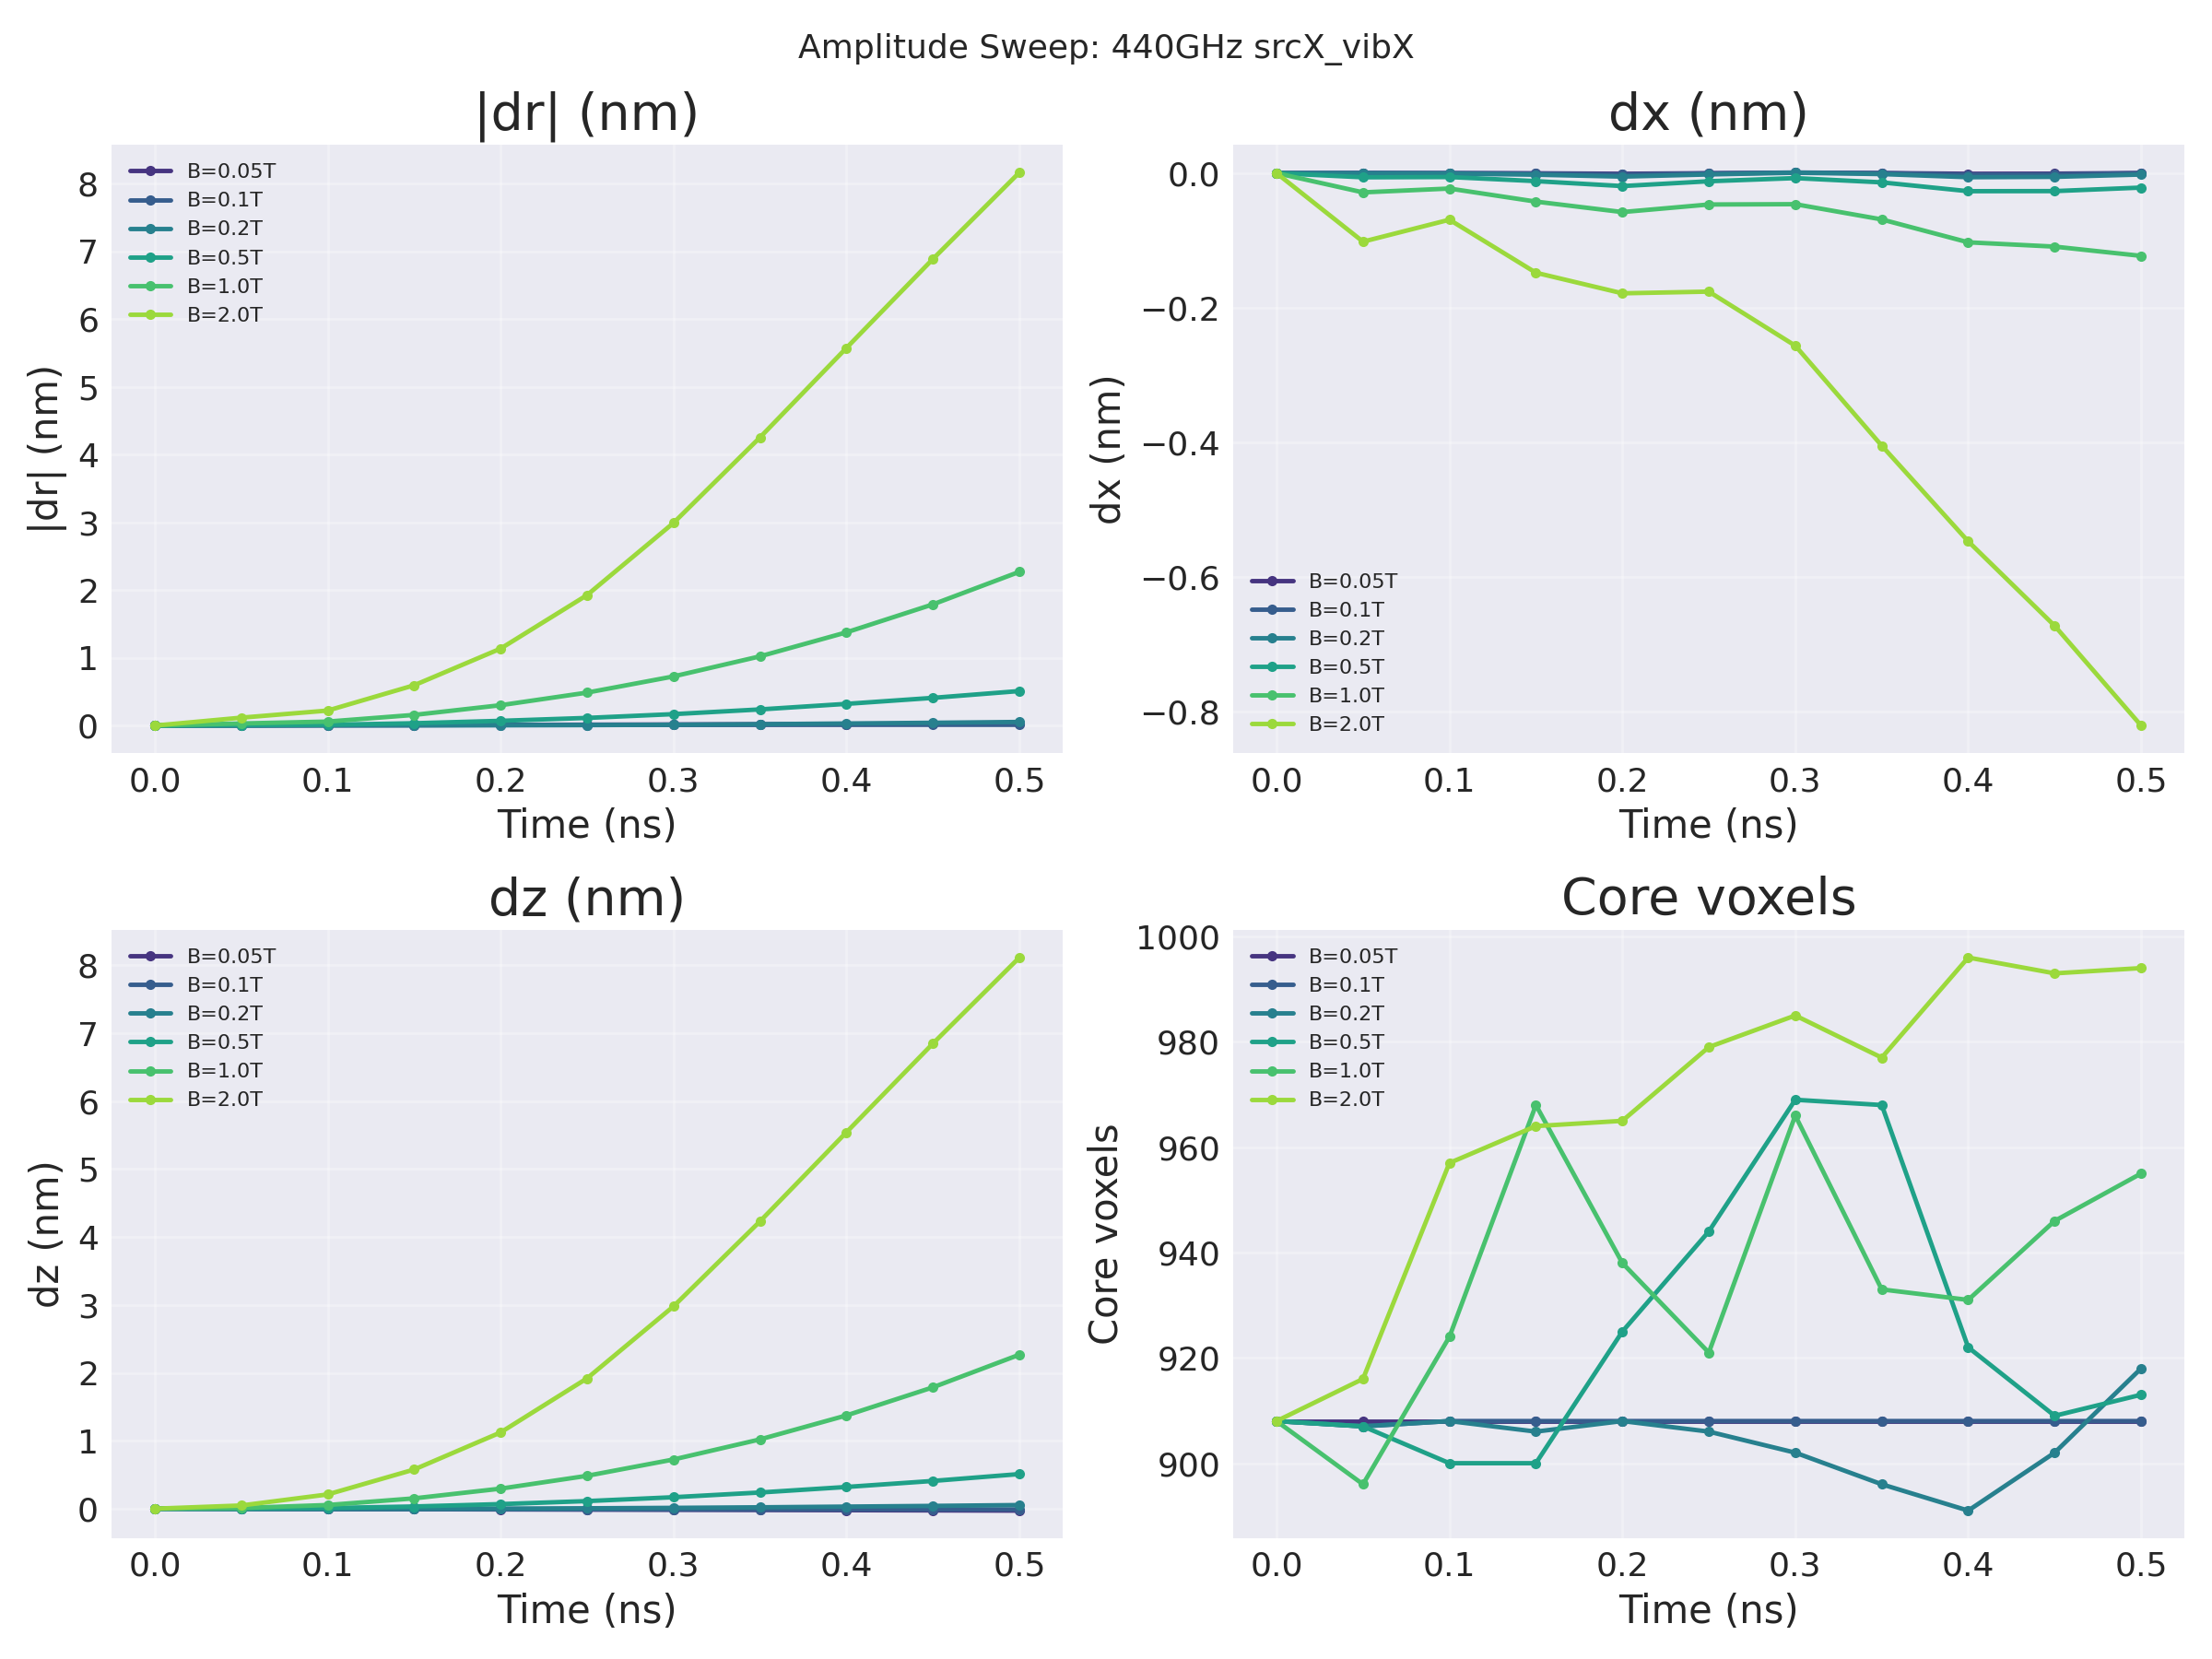
\includegraphics[width=0.95\textwidth]{figures/fig4-8_amplitude_trajectory.png}
  \caption{不同驱动幅度下 Hopfion 质心轨迹的对比结果}
  \label{fig:amplitude-trajectory}
\end{figure}

如\cref{fig:amplitude-scaling}所呈现，处于有效驱动窗口（$B_0 \geq \SI{0.5}{T}$）时，速度与幅度之间遵循幂律形式：
\begin{equation}
  \bar{v} = A \cdot B_0^n, \quad n = 1.99 \pm 0.01, \quad R^2 = 0.998
  \label{eq:amplitude-scaling}
\end{equation}
指数 $n \approx 2$ 具有清晰的物理含义：自旋波承载的线性动量密度正比于其能量密度 $\propto B_0^2$；Hopfion 的稳态速度由动量注入率与耗散率的平衡决定，故有 $v \propto B_0^2$。该标度律与 Skyrmion 自旋波驱动所得的 $v \propto B_0^2$ 一致\cite{ding2015motion}。

进入弱驱动极限（$B_0 \leq \SI{0.1}{T}$）后，Hopfion 位移跌至噪声量级（$|\Delta r| < \SI{0.1}{nm}$），表明系统存在阈值效应。$B_0 = \SIrange{0.05}{0.1}{T}$ 甚至出现朝源方向的微弱反向位移，这可能与低幅度下 Hopfion 的弹性反弹行为有关。

\par\noindent\textbf{拓扑 Hall 效应}\par\nobreak

在 srcX 驱动下，Hopfion 并非沿自旋波传播方向（$+x$）移动，而是几乎垂直于传播方向、朝 $+z$ 方向推进。本文将拓扑 Hall 角定义为 $\theta_{\text{H}} = \arctan(v_\perp / v_\parallel)$：其中 $v_\perp$ 指垂直于源平面的速度分量，$v_\parallel$ 则平行于传播方向。

\begin{figure}[htbp]
  \centering
  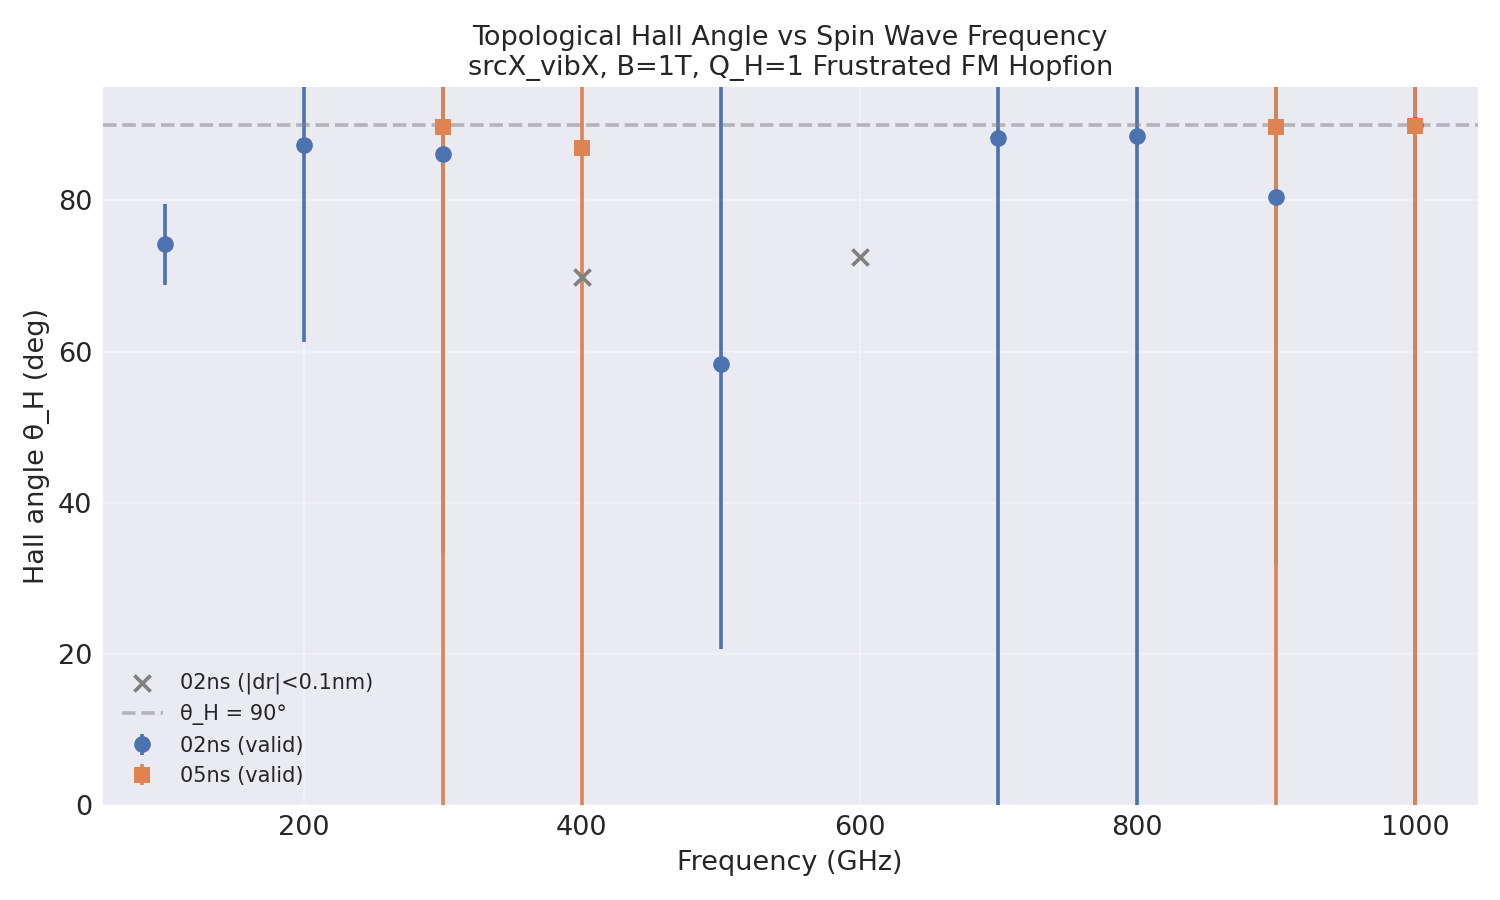
\includegraphics[width=0.95\textwidth]{figures/fig4-9_hall_angle_freq.png}
  \caption{拓扑 Hall 角 $\theta_{\text{H}}$ 的频率依赖曲线。有效驱动频率下 $\theta_{\text{H}} \approx \ang{87}$--$\ang{90}$，呈现拓扑保护特征}
  \label{fig:hall-angle-freq}
\end{figure}

从\cref{fig:hall-angle-freq}可见，对所有满足 $|\Delta r| > \SI{0.3}{nm}$ 的有效驱动频率，srcX 所对应的 Hall 角均聚集于 $\theta_{\text{H}} \approx \ang{87}$--$\ang{90}$，意味着 Hopfion 几乎完全沿传播方向的垂直分量前进。

\begin{figure}[htbp]
  \centering
  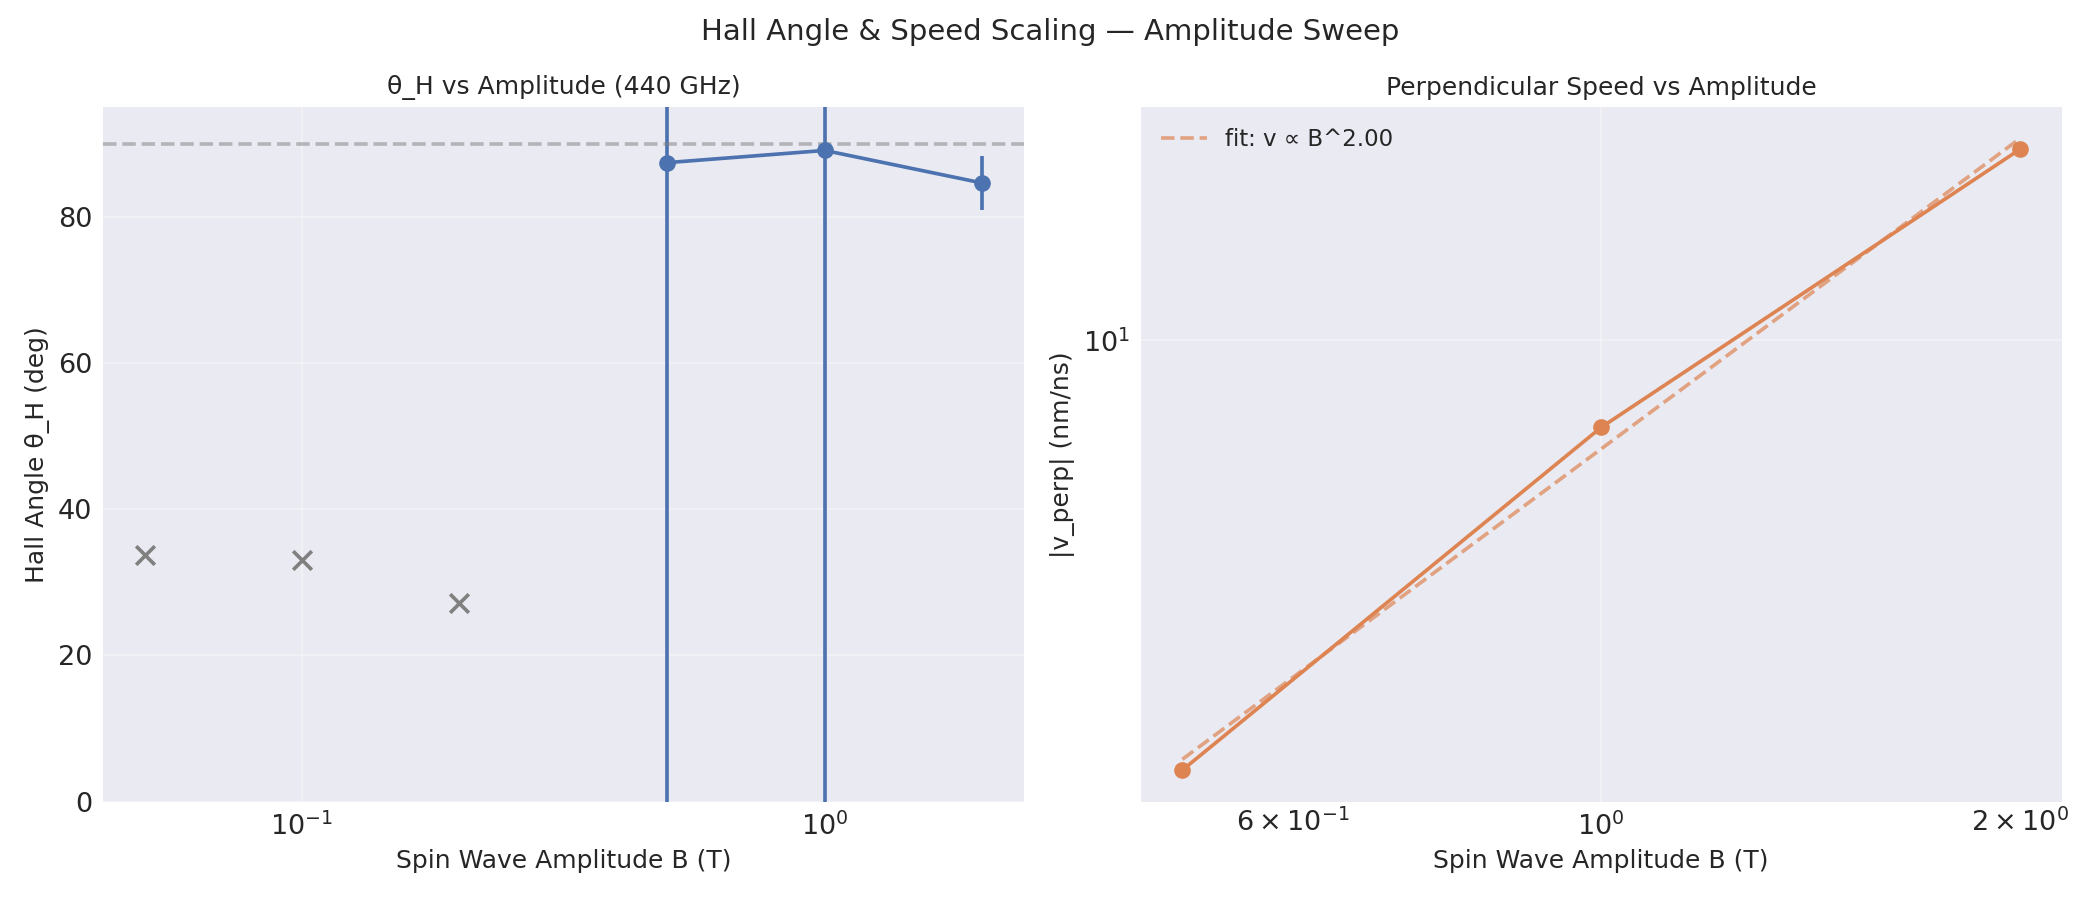
\includegraphics[width=0.95\textwidth]{figures/fig4-9b_hall_angle_amplitude.png}
  \caption{$f = \SI{440}{GHz}$ 固定下，拓扑 Hall 角（左）与垂直速度（右）对自旋波幅度的依赖。$B_0 \geq \SI{0.5}{T}$ 区段 Hall 角锁定在 $\ang{87}$--$\ang{90}$，弱驱动下因位移接近噪声水平而出现偏离}
  \label{fig:hall-angle-amplitude}
\end{figure}

\cref{fig:hall-angle-amplitude}进一步刻画了 Hall 角对驱动幅度的依赖。在有效驱动段（$B_0 \geq \SI{0.5}{T}$）内，Hall 角稳定维持于 $\ang{87}$--$\ang{90}$，对幅度变化不敏感。此种稳定性同时覆盖频率与幅度两个维度，直接佐证了 Hopfion 磁振子 Hall 效应具有拓扑保护特性——Hall 角的取值受制于拓扑结构本身，而非驱动条件的局部细节。

与之形成对照，srcZ 驱动推动 Hopfion 沿 $-z$（即传播方向）迁移，对应 $\theta_{\text{H}} \approx \ang{1}$，Hall 角几乎归零。两种驱动几何下 Hall 角的落差显著（srcX 的 $\ang{90}$ 对 srcZ 的 $\ang{1}$）。究其原因，面内自旋波经由动量转移在 Hopfion 势阱中产生等效横向力，其作用类似于二维 Skyrmion 中的 Magnus 力\cite{saji2023magnonic}；轴向自旋波则沿 Hopfion 对称轴施力，无法激发横向响应。

\par\noindent\textbf{双向轴向控制}\par\nobreak

综合前文数据可知，srcX 推动 $+z$、srcZ 推动 $-z$，对应的 Hall 角分别为 $\ang{90}$ 与 $\ang{1}$。换言之，只要切换自旋波的传播方向，即可在 $z$ 轴上实现 Hopfion 的双向可控迁移。此外，srcZ 在频率域上的方向异常（$\SI{100}{GHz}$ 对 $+z$，$\SI{1100}{GHz}$ 对 $-z$）还提示出另一条控制路径：保持单一 srcZ 源不变，仅通过频率切换便可触发方向反转。

\begin{figure}[htbp]
  \centering
  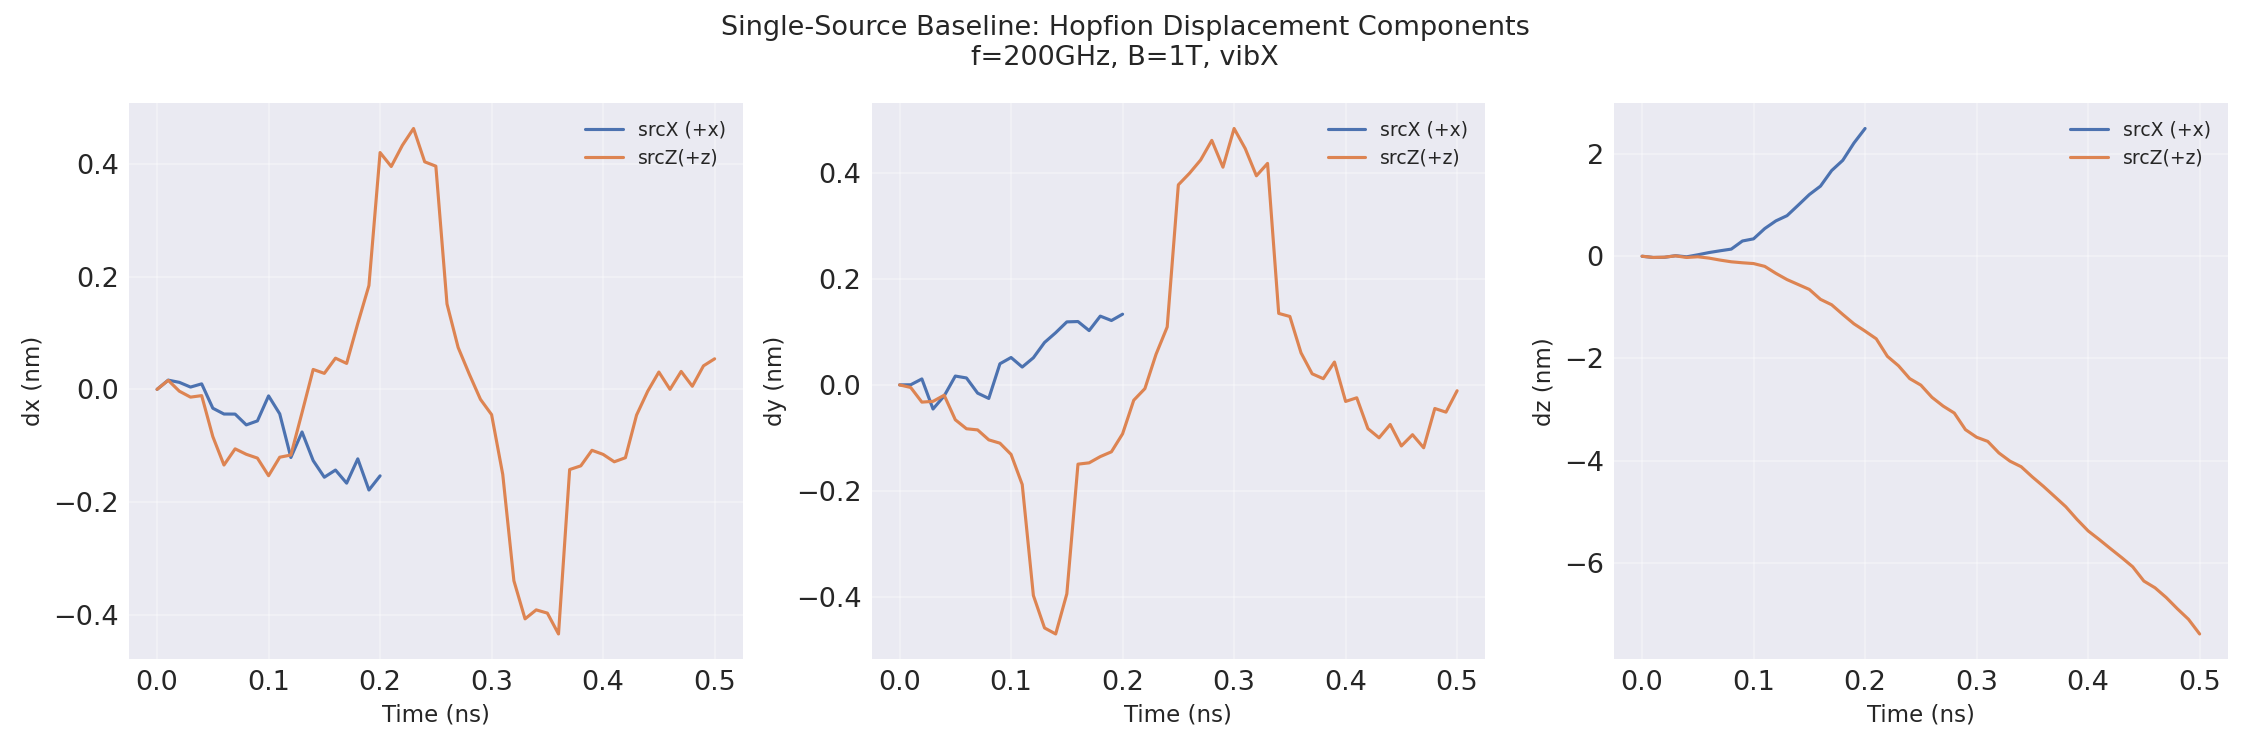
\includegraphics[width=0.95\textwidth]{figures/fig4-10_multisource_baseline.png}
  \caption{三种单源基线的 Hopfion 轨迹对比。srcX（$\SI{200}{GHz}$）驱动 $+z$，srcZ（$\SI{200}{GHz}$）驱动 $-z$，二者对应的 Hall 角分别为 $\ang{87}$ 与 $\ang{1}$}
  \label{fig:multisource-baseline}
\end{figure}

\cref{fig:multisource-baseline}对 srcX 与 srcZ 两类单源基线的运动轨迹作了定量对照，清晰呈现出两种驱动方向上的互补性。

为验证频率切换这一方案，本文设置了分时序仿真实验（v3 平衡时序）：Phase~1（$0$--$\SI{0.50}{ns}$）施加 srcZ@$\SI{100}{GHz}$，驱动 $+z$ 方向迁移；Phase~2（$\SI{0.50}{}$--$\SI{1.00}{ns}$）切换到 srcZ@$\SI{1100}{GHz}$，对应 $-z$ 方向运动。

从仿真结果来看（见\cref{fig:freq-switch-z}），Phase~1 期间 Hopfion 稳步向 $+z$ 移动，累计位移达到 $\SI{+17.6}{nm}$——$\SI{100}{GHz}$ 下 50 个完整周期为动量转移提供了足够的时间。进入 Phase~2 后，频率切换为 $\SI{1100}{GHz}$，Hopfion 随即反转为 $-z$ 方向运动，在 $\SI{0.41}{ns}$ 内从 $+\SI{17.6}{nm}$ 迅速移至 $-\SI{12.9}{nm}$（Phase~2 净位移 $\SI{-30.5}{nm}$），随后因持续强驱动触发拓扑结构失稳而坍塌。

该实验证实了单一 srcZ 源借助频率切换即可完成 Hopfion 运动方向的彻底反转。$-z$ 方向的速度（$\sim\SI{74}{nm/ns}$）明显超过 $+z$（$\sim\SI{35}{nm/ns}$），反映出两种频率耦合强度上的差异。Phase~2 后期的坍塌现象则提示，强自旋波驱动下拓扑结构的寿命本身存在上限；实际应用中需对驱动幅度加以优化或引入脉冲调制，从而在速度与寿命之间取得平衡。

\begin{figure}[htbp]
  \centering
  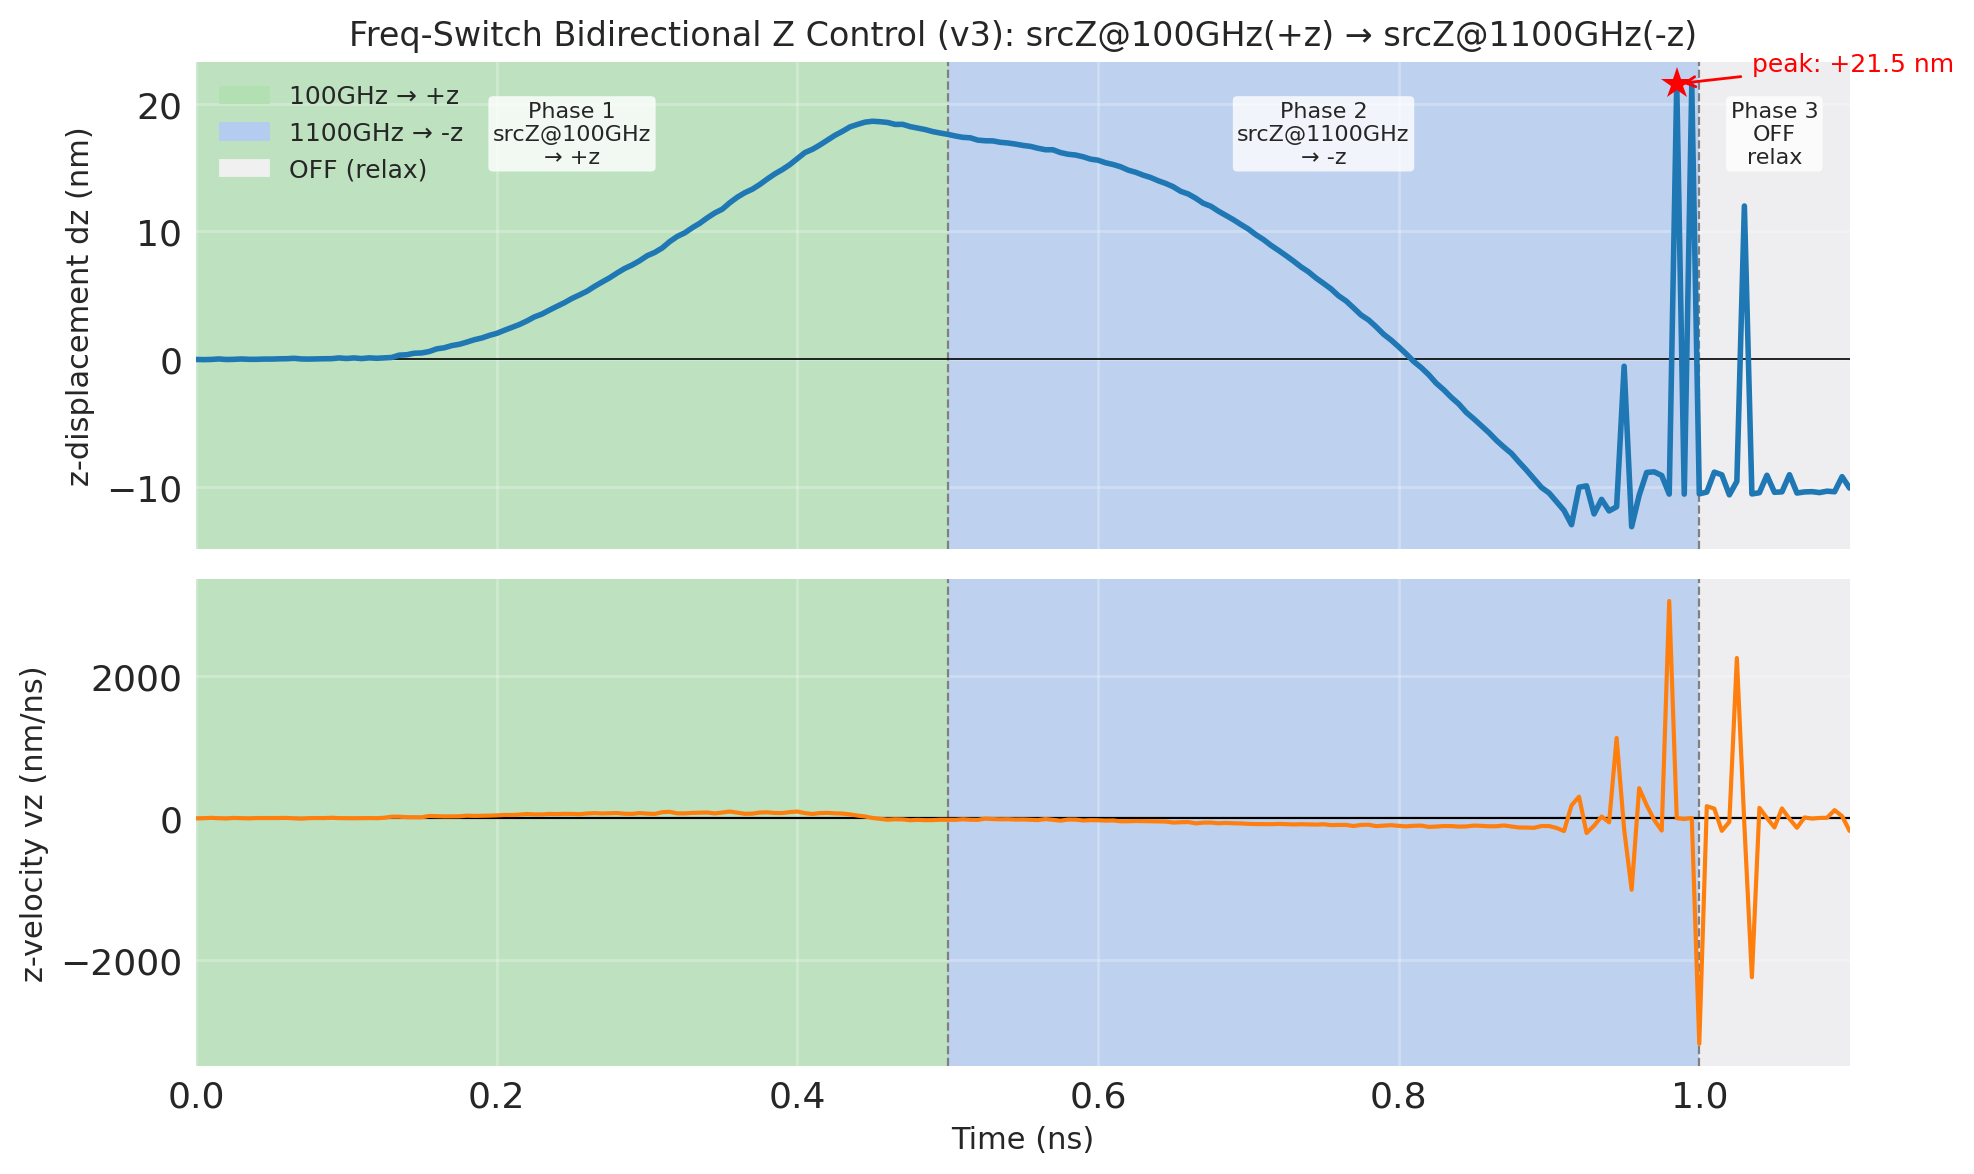
\includegraphics[width=0.95\textwidth]{figures/fig4-11_freq_switch_z_control.png}
  \caption{频率切换下双向 $z$ 轴控制的验证结果（v3 平衡时序）。上：$z$ 方向位移对时间的变化；下：$z$ 方向速度。绿色区对应 srcZ@$\SI{100}{GHz}$（$0$--$\SI{0.50}{ns}$，$+z$），蓝色区对应 srcZ@$\SI{1100}{GHz}$（$\SI{0.50}{}$--$\SI{1.00}{ns}$，$-z$）。Hopfion 在 $t \approx \SI{0.91}{ns}$ 因强驱动而坍塌}
  \label{fig:freq-switch-z}
\end{figure}

\par\noindent\textbf{与二维 Skyrmion 自旋波驱动的对比}\par\nobreak

Hopfion 的自旋波驱动机制与二维 Skyrmion 的情形具有自然的类比关系。Ding 等\cite{ding2015motion}与 Huang 等\cite{huang2023transient}指出，自旋波通过线性动量转移推动 Skyrmion 沿传播方向迁移，速度受频率与振幅共同调制。回旋矢量为零的 Skyrmionium 亦被 Shen 等\cite{shen2018skyrmionium}考察，其沿自旋波传播方向做直线运动、无霍尔偏转——这一特征恰与 Hopfion 的 $\mathbf{G} = 0$ 属性相呼应。

本章仿真与上述二维体系的共性与差异可归纳为以下几点：

\begin{enumerate}
  \item \textbf{幅度标度律一致}：Hopfion 所得 $v \propto B_0^{1.99}$ 与 Skyrmion/Skyrmionium 的 $v \propto B_0^2$ 相互吻合，这说明三维拓扑结构下动量转移的基本机制并未发生改变。
  \item \textbf{Hall 角差异}：二维 Skyrmion 的 Hall 角取决于拓扑荷 $Q$ 与耗散张量，典型取值范围为 $\ang{0}$--$\ang{60}$。相比之下，Hopfion 在 srcX 驱动下获得 $\theta_{\text{H}} \approx \ang{90}$ 的极端 Hall 角——此类取值在二维系统中实属罕见，反映出三维拓扑结构所具备的独特耦合通道。Saji 等人\cite{saji2023magnonic}曾从解析层面预言过类似的磁振子 Hall 效应，本章仿真则在微磁学尺度首次给出定量验证。
  \item \textbf{三维新自由度}：二维 Skyrmion 受限于面内运动，而 Hopfion 的三维构型额外提供轴向自由度。srcX 与 srcZ 分别激活面内-轴向耦合通道和直接轴向通道，使得单一体系即可实现双向控制——该功能在二维拓扑结构中无从实现。
  \item \textbf{振荡方向选择性}：二维体系的 Skyrmion 对自旋波的面内/面外振荡均有响应\cite{ding2015motion}，而 Hopfion 仅对面内振荡敏感，面外振荡完全无效。这种选择性根源于 Hopfion 的轴对称拓扑结构。
\end{enumerate}

\par\noindent\textbf{点源与平面源的对比}\par\nobreak

前述各项仿真皆以平面波激励（$\SI{0.5}{nm}$ 厚薄片层，$B_0 = \SI{1}{T}$）为前提。为评估激励几何对驱动行为的影响，本文补充了点源对照实验：激励区域收缩至单个网格单元（$\SI{0.5}{nm}^3$，位于同一坐标），幅度则相应增至 $B_0 = \SI{500}{T}$ 以补偿体积差别，其余参数维持不变。沿 srcX、srcZ 两种传播方向各进行 $\SIrange{100}{1000}{GHz}$ 的 10 点频率扫描。

\begin{figure}[htbp]
  \centering
  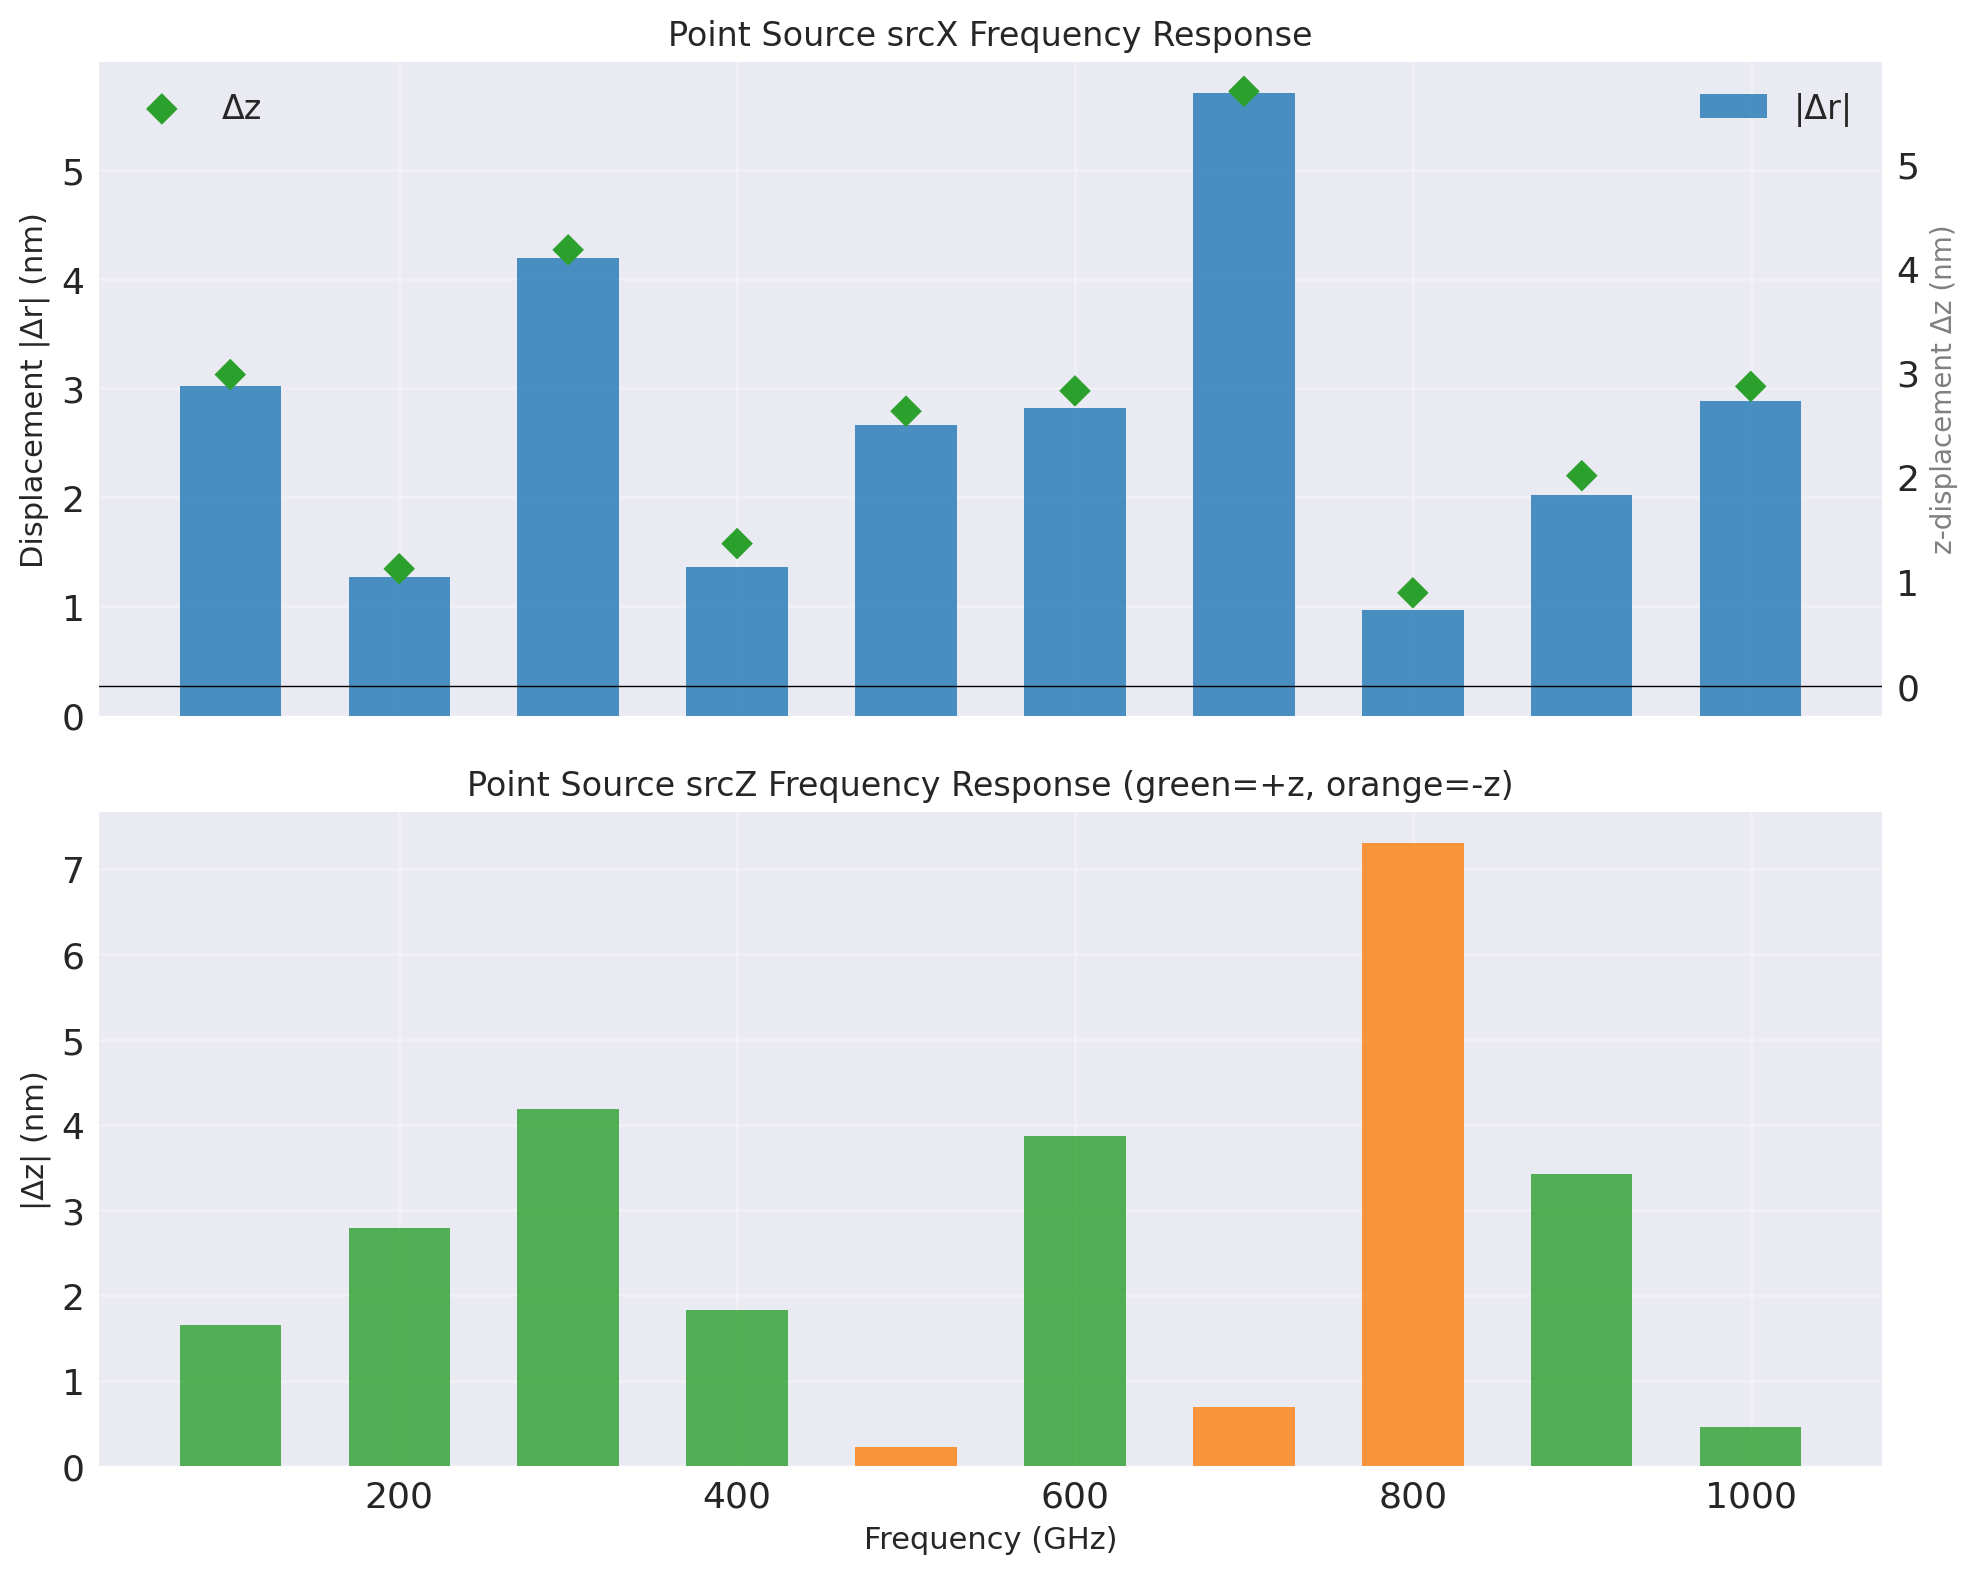
\includegraphics[width=0.95\textwidth]{figures/fig4-12_point_source_freq_response.png}
  \caption{点源驱动下的频率响应谱。上图 srcX：最强响应出现于 $\SI{700}{GHz}$（$|\Delta r| = \SI{5.7}{nm}$）；下图 srcZ：最强响应位于 $\SI{800}{GHz}$（$|\Delta r| = \SI{7.3}{nm}$，$-z$）；绿色、橙色分别代表 $+z$、$-z$ 方向}
  \label{fig:point-source-freq}
\end{figure}

从\cref{fig:point-source-freq}可见，点源驱动与平面源之间的差别相当明显：

\begin{enumerate}
  \item \textbf{共振频率偏移}：srcX 的峰值频率由平面源的 $\SI{1000}{GHz}$ 移至 $\SI{700}{GHz}$（$|\Delta r| = \SI{5.7}{nm}$），原有死区不复存在；srcZ 的峰值频率则从 $\SI{1100}{GHz}$ 移至 $\SI{800}{GHz}$（$|\Delta r| = \SI{7.3}{nm}$）。这种移动可归咎于点源激发的自旋波所含波矢分布更宽，由此改变了与 Hopfion 内模的耦合条件。
  \item \textbf{方向特征保持}：srcX 点源对应的 10 个频率全部驱动 $+z$ 运动，与平面源结果一致。srcZ 的方向分布则复杂得多——100--$\SI{400}{GHz}$、$\SI{600}{GHz}$、$\SI{900}{GHz}$ 为 $+z$，$\SI{500}{GHz}$、$\SI{700}{GHz}$、$\SI{800}{GHz}$ 为 $-z$——平面源中仅 $\SI{100}{GHz}$ 表现为方向异常，点源情形下则有多个频率出现反转。
  \item \textbf{Hall 角鲁棒性}：从\cref{fig:point-source-hall}可见，srcX 点源的 Hall 角仍然聚集在 $\ang{69}$--$\ang{89}$，高 Hall 角的拓扑特征得以保留。srcZ 的 Hall 角则由平面源的 $\approx\ang{1}$ 扩展到 $\ang{9}$--$\ang{40}$，这意味着点源的非对称激励部分地破坏了轴向对称性，引入了弱横向耦合成分。
\end{enumerate}

\begin{figure}[htbp]
  \centering
  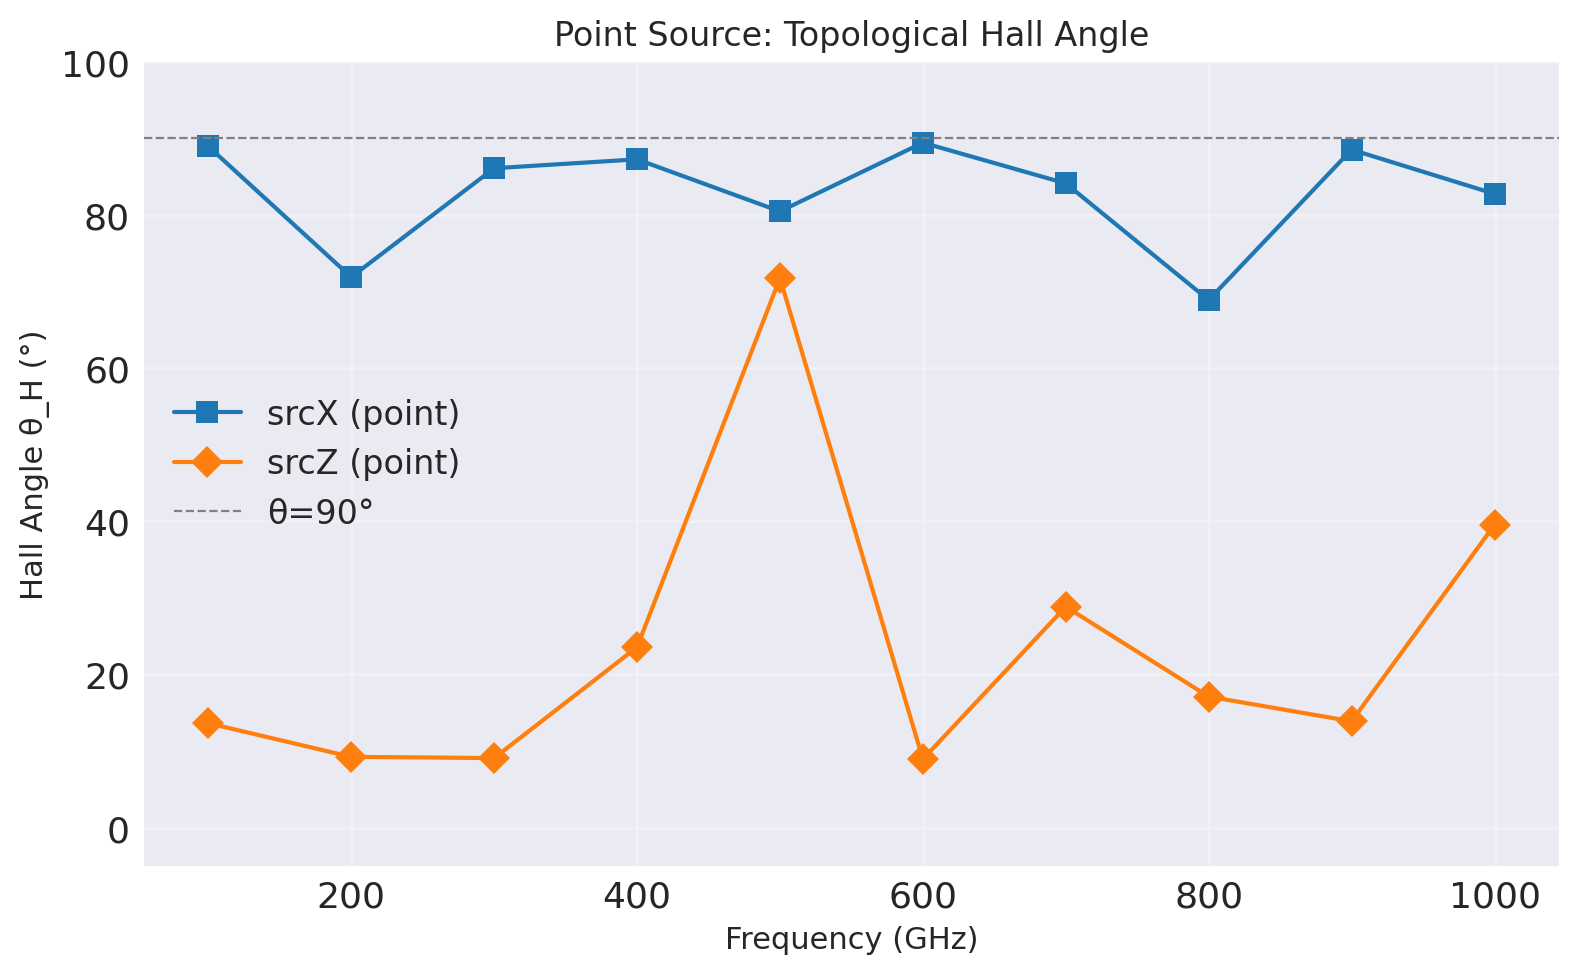
\includegraphics[width=0.85\textwidth]{figures/fig4-13_point_source_hall_angle.png}
  \caption{点源与平面源 Hall 角的比较。srcX 的高 Hall 角（$\ang{69}$--$\ang{89}$）得以保留，srcZ 则由 $\approx\ang{1}$ 抬升至 $\ang{9}$--$\ang{40}$}
  \label{fig:point-source-hall}
\end{figure}

上述对照说明，Hopfion 对自旋波响应的核心特征——振荡方向选择性、运动方向以及高 Hall 角——本质上由其拓扑结构决定，与激励几何的具体细节无关。点源虽然改变了共振频率与方向分布的细节面貌，却未触动整体物理图像。


自旋波驱动 Hopfion 运动的物理机制，本章经由平面源与点源两条路线完成了比较完整的刻画，六项核心发现分述如下：

\begin{enumerate}
  \item \textbf{方向选择性}：面内振荡（vibX）自旋波是驱动 Hopfion 运动的有效激发源，面外振荡（vibZ）则无响应；面内传播方向（srcX/srcY）之间的各向同性结果，从侧面佐证了 Hopfion 的轴对称性。
  \item \textbf{频率响应}：srcX 的最大位移出现在 $\SI{1000}{GHz}$（$|\Delta r| = \SI{5.5}{nm}$），$\SIrange{400}{600}{GHz}$ 对应明显死区；srcZ 的最强响应则推至 $\SI{1100}{GHz}$（$|\Delta r| = \SI{18.1}{nm}$），并伴随多峰共振结构。一处例外值得单独提出：srcZ 在 $\SI{100}{GHz}$ 处沿 $+z$ 运动，其余频率全部指向 $-z$。
  \item \textbf{幅度标度律}：Hopfion 的运动速度与自旋波幅度 $B_0$ 之间呈现幂律关系 $v \propto B_0^{1.99}$（$R^2 = 0.998$），与动量转移理论所预言的指数吻合良好。
  \item \textbf{拓扑 Hall 效应}：srcX 激发下的 Hall 角 $\theta_{\text{H}} \approx \ang{87}$--$\ang{90}$，在频率与幅度两轮扫描中均表现出高度稳定性，属于典型的拓扑保护行为；相较之下，srcZ 对应的 Hall 角仅约 $\ang{1}$，运动基本沿传播方向进行。
  \item \textbf{双向控制}：srcX 走 $+z$ 而 srcZ 走 $-z$，两条路径本身已构成方向互补；srcZ 自身的频率相关方向异常则进一步提供了单激励源内部的双向切换可能，使 Hopfion 在 $z$ 轴方向的可控迁移具备两种独立实现路径。
  \item \textbf{激励几何鲁棒性}：点源与平面源两类激励的对照结果说明，振荡方向选择性以及高 Hall 角这两项关键特征的根源在于 Hopfion 的拓扑结构本身，对激励几何的具体细节并不敏感。
\end{enumerate}
